\documentclass[9pt]{beamer}

\usepackage{ucs}
\usepackage[utf8x]{inputenc}
% \usepackage{beamerthemeplain}

\usepackage{amsmath}
\usepackage{amsfonts}
\usepackage{amssymb}
\usepackage[english]{babel}
\usepackage{fontenc}
% \usepackage{verbatim}
\usepackage{graphics}
 
\usepackage{textcomp}
\usepackage[absolute,overlay]{textpos}

\usepackage{wasysym}

\usepackage{slashed}
\usepackage{array}

\usetheme{CNRScolors}

\newcommand{\afac}[1]{\noindent \textcolor{red}{{\small \sc #1}}}

\usepackage{xspace}
%units
\usepackage[squaren,Gray,mediumqspace,thinspace,textstyle]{SIunits}

\usepackage[permil]{overpic}

\usepackage{textcomp}
\usepackage[absolute,overlay]{textpos}

\newcommand{\egamma}{E_{\gamma}}
\newcommand{\unitMass}{\giga\electronvolt/c^2}
\newcommand{\unitMom}{\giga\electronvolt/c}
\newcommand{\GeV}{\giga\electronvolt}
\newcommand{\TeV}{\tera\electronvolt}
\newcommand{\fb}{\femto\barn}
\newcommand{\pb}{\pico\barn}
\newcommand{\invmub}{\micro\reciprocal\barn}
\newcommand{\invpb}{\pico\reciprocal\barn}
\newcommand{\invfb}{\femto\reciprocal\barn}
\newcommand{\invnb}{\nano\reciprocal\barn}
\newcommand{\lumi}{\ensuremath{\mathcal{L}}}
\newcommand{\lumiunit}{\centi\meter\rpsquared\usk\reciprocal\second}
\newcommand{\pomeron}{\mathbb{P}}
\newcommand{\xp}{x_\pomeron}
\newcommand{\dkap}{\ensuremath{\Delta\kappa^{\gamma}}}
\newcommand{\kap}{\ensuremath{\kappa^{\gamma}}}
\newcommand{\lam}{\ensuremath{\lambda^{\gamma}}}
\newcommand{\aOw}{\ensuremath{a_0^W}}
\newcommand{\aOz}{\ensuremath{a_0^Z}}
\newcommand{\aCw}{\ensuremath{a_C^W}}
\newcommand{\aCz}{\ensuremath{a_C^Z}}
\newcommand{\aOwL}{\ensuremath{a_0^W/\Lambda^2}}
\newcommand{\aOzL}{\ensuremath{a_0^Z/\Lambda^2}}
\newcommand{\aCwL}{\ensuremath{a_C^W/\Lambda^2}}
\newcommand{\aCzL}{\ensuremath{a_C^Z/\Lambda^2}}
% \newcommand{\Lcutoff}{\ensuremath{\Lambda_{\text{cutoff}}}}
\newcommand{\Lcutoff}{\ensuremath{\Lambda}}
\newcommand{\wwgamma}{WW\gamma}
\newcommand{\missET}{\ensuremath{\not\!\!E_T}}
\newcommand{\etmiss}{\ensuremath{\not\!\!E_T}}
\newcommand{\WWgg}{\ensuremath{WW\gamma\gamma}}
\newcommand{\ggWW}{\ensuremath{WW\gamma\gamma}}
\newcommand{\dd}{\mathop{}\mathopen{}\text{d}}

\newcommand{\gpU}[1]{\ensuremath{\text{U}({#1})}}
\newcommand{\gpSU}[1]{\ensuremath{\text{SU}({#1})}}
\newcommand{\gpO}[1]{\ensuremath{\text{O}({#1})}}
\newcommand{\gpSO}[1]{\ensuremath{\text{SO}({#1})}}

\newcommand{\DO}{D\O{}\xspace}

\newcommand{\ith}{\textsuperscript{th}}
\newcommand{\st}{\textsuperscript{st}}
\newcommand{\nd}{\textsuperscript{nd}}
\newcommand{\rd}{\textsuperscript{rd}}

% \myfig[width=3cm]{label}{images/Chap1/myfig.pdf}{The capture of my figure.}
\newcommand{\myfig}[4][width=0.7\textwidth]{%
\begin{center}
 \begin{figure}
  \includegraphics[#1]{#3}
  
 \caption{\label{#2} #4}
 \end{figure}
\end{center}
}

\newcommand\FrameText[1]{%
  \begin{textblock*}{\paperwidth}(0pt,33pt)
    \raggedleft \small #1\hspace{.5em}
  \end{textblock*}}

\newcommand{\myincgr}[4]{
     \begin{overpic}[#1]{#2}
     \put(#3){#4}
     \end{overpic}}
\newcommand{\myincgrduo}[6]{
     \begin{overpic}[#1]{#2}
     \put(#3){#4}
     \put(#5){#6}
     \end{overpic}}
{\newcommand{\cmsSymbolFace}{\text}
\newcommand{\PT}{\ensuremath{p_{\text{T}}}\xspace}
\newcommand{\pt}{\ensuremath{p_{\text{T}}}\xspace}
\newcommand{\cm}{\ensuremath{\,\text{cm}}\xspace}
\newcommand{\PGm}{\ensuremath{\mu}\xspace} % muon
% \newcommand{\GeV}{\ensuremath{{\,\text{Ge\hspace{-.08em}V}}}\xspace}
\newcommand{\GeVc}{\ensuremath{{\,\text{Ge\hspace{-.08em}V\hspace{-0.16em}/\hspace{-0.08em}}c}}\xspace}
\newcommand{\GeVcc}{\ensuremath{{\,\text{Ge\hspace{-.08em}V\hspace{-0.16em}/\hspace{-0.08em}}c}^2}\xspace}
\newcommand{\abs}[1]{\ensuremath{\lvert #1 \rvert}}

% frequently used expressions
\newcommand{\ee}{\ensuremath{e^+e^-}\xspace}
\newcommand{\mumu}{\ensuremath{\mu^+\mu^-}\xspace}
\newcommand{\Mmumu}{\ensuremath{m_{\mu\mu}}\xspace}
\newcommand{\mmumu}{\ensuremath{m_{\mu\mu}}\xspace}
\newcommand{\eexp}[1]{\ensuremath{{\text e}^{#1}}\xspace}

% \newcommand{\qqbar}{\ensuremath{{\cmsSymbolFace{q}\overline{\cmsSymbolFace{q}}}}\xspace}
\newcommand{\QQbar}{\ensuremath{{\cmsSymbolFace{Q}\overline{\cmsSymbolFace{Q}}}}\xspace}
\newcommand{\Jpsi}{\ensuremath{\cmsSymbolFace{J}\hspace{-.08em}/\hspace{-.14em}\psi}\xspace}
\newcommand{\JPsi}{\ensuremath{\cmsSymbolFace{J}\hspace{-.08em}/\hspace{-.14em}\psi}\xspace}
\newcommand{\psiP}{\ensuremath{\psi\text{(2S)}}\xspace}
\newcommand{\B}{\ensuremath{\cmsSymbolFace{B}}\xspace}
\newcommand{\D}{\ensuremath{\cmsSymbolFace{D}}\xspace}

% \newcommand{\doubleRatio}{\ensuremath{\left.\left[N_{\psiP}/N_{\Jpsi}\right]_{\PbPb}\middle/\left[N_{\psiP}/N_{\Jpsi}\right]_{\pp}\right.\xspace}}
\newcommand{\doubleRatio}{\ensuremath{\left.(N_{\psiP}/N_{\Jpsi})_{\PbPb}/(N_{\psiP}/N_{\Jpsi})_{\pp}\right.\xspace}}

\newcommand{\PgU}{\ensuremath{\Upsilon}\xspace}
\newcommand{\PgUa}{\ensuremath{\Upsilon\text{(1S)}}\xspace}
\newcommand{\PgUb}{\ensuremath{\Upsilon\text{(2S)}}\xspace}
\newcommand{\PgUc}{\ensuremath{\Upsilon\text{(3S)}}\xspace}
\newcommand{\PgUbc}{\ensuremath{\Upsilon\text{(2S+3S)}}\xspace}
\newcommand{\PgUabc}{\ensuremath{\Upsilon\text{(1S,2S,3S)}}\xspace}
\newcommand{\PgUn}{\ensuremath{\Upsilon\text{(nS)}}\xspace}

\newcommand{\W}{\ensuremath{\cmsSymbolFace{W}}\xspace}
%\newcommand{\Z}{\ensuremath{\cmsSymbolFace{Z}}\xspace}
\newcommand{\ttbar}{\ensuremath{\cmsSymbolFace{t}\bar{\cmsSymbolFace{t}}}\xspace}

\newcommand{\dndy}{\ensuremath{dN/dy}\xspace}
\newcommand{\dnchdy}{\ensuremath{dN_{\text{ch}}/dy}\xspace}
\newcommand{\dndeta}{\ensuremath{dN/d\eta}\xspace}
\newcommand{\dnchdeta}{\ensuremath{dN_{\text{ch}}/d\eta}\xspace}
\newcommand{\dndpt}{\ensuremath{dN/d\pt}\xspace}
\newcommand{\dnchdpt}{\ensuremath{dN_{\text{ch}}/d\pt}\xspace}
\newcommand{\deta}{\ensuremath{\Delta\eta}\xspace}
\newcommand{\dphi}{\ensuremath{\Delta\phi}\xspace}
\newcommand{\phistar}{\ensuremath{\phi^*}\xspace}

\newcommand {\npart}  {\ensuremath{N_{\text{part}}}\xspace}
\newcommand {\ncoll}  {\ensuremath{N_{\text{coll}}}\xspace}

\newcommand{\AAA}{\ensuremath{\text{AA}}\xspace}
\newcommand{\raa}{\ensuremath{R_{\AAA}}\xspace}
\newcommand{\rpa}{\ensuremath{R_{\text{pA}}}\xspace}
\newcommand{\taa}{\ensuremath{T_{\AAA}}\xspace}
\newcommand{\rfb}{\ensuremath{R_\text{FB}}\xspace}

% references to equations, figures or tables
\newcommand{\eq}[1]{Eq.~\eqref{#1}\xspace}
\newcommand{\fig}[1]{Fig.~\ref{#1}\xspace}
\newcommand{\tab}[1]{Table~\ref{#1}\xspace}

% collision types
\newcommand{\pp}{{\ensuremath{\text{pp}}}\xspace}
\newcommand{\ppbar}{\ensuremath{\text{p}\overline{\text{p}}}\xspace}
\newcommand{\pPb}{\ensuremath{\text{p}\text{Pb}}\xspace}
\newcommand{\ppb}{\ensuremath{\text{p}\text{Pb}}\xspace}
\newcommand{\PbPb}{\ensuremath{\text{PbPb}}\xspace}
\newcommand{\pbpb}{\ensuremath{\text{PbPb}}\xspace}
\newcommand{\AuAu}{\ensuremath{\text{AuAu}}\xspace}

% center of mass energy
\newcommand{\sqrts}{\ensuremath{\sqrt{s}}\xspace}
\newcommand{\sqrtsnn}{\ensuremath{\sqrt{s_{_{\text{NN}}}}}\xspace}

%units
\newcommand{\mbinv} {\mbox{\ensuremath{\,\text{mb}^\text{$-$1}}}\xspace}
%\newcommand{\mubinv} {\mbox{\ensuremath{\,\mu\text{b}^\text{$-$1}}}\xspace}

% program name
\providecommand{\CASCADE} {{\textsc{cascade}}\xspace}
\providecommand{\HYDJET} {{\textsc{hydjet}}\xspace}


% ljpsi
\newcommand{\Lxy}{\ensuremath{L_{xy}}\xspace}
\newcommand{\Lxyz}{\ensuremath{L_{xyz}}\xspace}
% \newcommand{\ctau}{\ensuremath{c\tau^{2D}}\xspace}
% \newcommand{\ctauxyz}{\ensuremath{c\tau^{3D}}\xspace}
\newcommand{\ctau}{\ensuremath{\ell_{\Jpsi}^{2D}}\xspace}
\newcommand{\ctauxyz}{\ensuremath{\ell_{\Jpsi}^{3D}}\xspace}

% pPb 
\newcommand{\etalab}{\ensuremath{\eta_\text{lab}}\xspace}

\graphicspath{ {../figures/}{./} }

\setbeamertemplate{navigation symbols}{}

 \newcolumntype{x}[1]{%
>{\centering\hspace{0pt}}p{#1}}%
\newcommand{\tn}{\tabularnewline}

\date[Stat1]{Sept. 20, 2018}
\title{Methods of statistical analysis and simulation}
\subtitle{Cours 1}
\author[E. Chapon]{Émilien Chapon}
% \institute[(CERN)]{CERN}
% \logo{\includegraphics[height=0.6cm]{../../CMS-Color-Label.pdf}\hspace{1.05\textwidth}\includegraphics[height=0.6cm]
% {../../LogoBadge.pdf} }

\begin{document}

{
\setbeamertemplate{footline}{}
\setbeamertemplate{headline}{}
% \logo{\includegraphics[height=1.2cm]{../../CMS-Color-Label.pdf}
% \hspace{0.94\textwidth}\includegraphics[height=1.2cm]{../../LogoBadge.pdf}}

\begin{frame}
 \maketitle
 
%  \setcounter{framenumber}{0}
\end{frame}
}

\begin{frame}
 \frametitle{Organisation of the class}
 
 \begin{block}{Organisation of the class}
  Two modules:
  
  \begin{itemize}
   \item Part 1: Methods of statistical analysis and simulation
   \begin{itemize}
    \item Émilien Chapon, $8\times 4$ hours
   \end{itemize}
   \item Part 2: Experiments and detector physics
   \begin{itemize}
    \item Jean-Claude Brient, $8\times 4$ hours
   \end{itemize}
  \end{itemize}

 \end{block}
 
 Exam for Methods of statistical analysis and simulation: TBD (likely article discussion)

\end{frame}

\section*{Introduction}

\begin{frame}
 \frametitle{Who am I?}
 
 \begin{itemize}
  \item Particle physicist at CERN
  \item CMS (general-purpose experiment at the CERN LHC)
  \item Studying heavy-ion collisions
  \item Graduated on the search for H$\to$WW at the Tevatron (D0)
 \end{itemize}

\end{frame}

\begin{frame}
 \frametitle{Contents of this course}
 
 \begin{itemize}
  \item Probability and random variables
  \item Parameter estimation
  \item Hypothesis testing
 \end{itemize}

\end{frame}

\begin{frame}
 \frametitle{Introduction}
 
 Introduction
\end{frame}

\begin{frame}
 \frametitle{Definitions are important}

 % Cousins slides, part 1 s5
 As in physics, much confusion can be avoided by being
precise about definitions, and much confusion can be
generated by being imprecise, or by assuming every-day
definitions in a technical context.

\begin{exampleblock}{Example}
 When you read: ``The confidence level tells you how much confidence one
has that the true value is in the confidence interval.''

$\to$ confusion on the ``usual'' and ``statistician'' meanings of the word confidence...

\end{exampleblock}

\end{frame}


\begin{frame}
 \frametitle{Language}
 
 \begin{center}
 \begin{tabular}{ll}
  Physicists say... & when Statisticians say... \\
  \hline
  Determine & Estimate \\
  Estimate & Guess \\
  Gaussian & Normal \\
  Breit-Wigner\footnote{This is what HEP physicists say. Others say Lorentzian...} & Cauchy \\
 \end{tabular}
 \end{center}
 
 (Side note: statistics is a field of mathematics, not a quantifier of data: avoid wishing for ``more statistics''...)
 

\end{frame}

\begin{frame}
 \frametitle{Key tasks in Statistics: important to distinguish!}
 
 \begin{description}
  \item<1->[Point estimation:] what single ``measured'' value of a parameter do you report?
  \item<2->[Interval estimation:] what interval (giving a measure of uncertainty of the parameter inference) do you report?
  \item<3->[Hypothesis testing:] Many special cases:
  \begin{enumerate}
   \item A given functional form (“model”) vs another functional
form. Also known as “model selection”.
  \item A single value of a parameter (say 0 or 1) vs all other values
  \item Goodness of Fit: A given functional form against all other
(unspecified) functional forms (aka “model checking”)
  \end{enumerate}
  \item<4>[Decision making:] What action should I take (tell no one, issue
press release, propose new experiment, ...) based on the
observed data? Rarely done formally in HEP, but important to
understand outline of formal theory, to avoid confusion with
inference and to inform informal application.
  \end{description}

\end{frame}

% \begin{frame}
%  \frametitle{Key tasks in Statistics: important to distinguish!}
%  
%  In frequentist statistics, the above hypothesis testing case,
%  
% \structure{(2) A single value of a parameter (say 0 or 1) vs all other values,}
% 
% maps identically onto interval estimation.
% 
% This is called the duality of “inversion of a hypothesis test to get
% confidence interval”, and vice versa, and will be discussed later.
% 
% In contrast, in Bayesian statistics, testing case (b) is an
% especially controversial form of case (a) model selection.
% The model with fixed value of parameter is lower-dimensional in
% parameter space than the model with parameter not fixed.
% 
% Again, I just mention this here to foreshadow a very deep issue,
% where frequentist and Bayesian methods do not converge in the
% limit of large data sets.
% 
% \end{frame}

\begin{frame}
 \frametitle{Two philosophies}
 
 Unfortunately, statisticians do not agree on basic principles. They can crudely be divided into two schools: Bayesian and frequentist (or classical). The name Bayesian
 derives from the extended use of Bayes theorem in the former group.
 
 \begin{block}{Bayesian}
  Closer to everyday reasoning, where probability is interpreted as a \emph{degree of belief} that something will happen, or that a parameter will have a given value. 
 \end{block}
 
 \begin{block}{Frequentist}
  Closer to scientific reasoning, where probability means the relative frenquency of something happening. This makes it more objective, since it can be determined independently of the 
  observer, but restricts its application to repeatable phenomena.
  
  In particular: one can define the frequentist probability for observing data (which are random), but not for the true value of a parameter (which is fixed, even if unknown).
 \end{block}


\end{frame}

\begin{frame}
 \frametitle{Frequentist vs Bayesian}
 
 In the areas of parameter estimation and hypothesis testing, numerical results tend to be the same with both approaches in the asymptotic regime (i.e. large data set).
 
 Differences do exist however (and can lead to ``paradoxes''):
 
 \begin{itemize}
  \item Exact frequentist results require as input the probabilities of observing all data, both the one actually measured and that which could have been observed (Monte-Carlo). This violates an important principle in Bayesian theory, and is not allwoed in the Bayesian method.
  \item Goodness-of-fit is essentially impossible to obtain in the Bayesian approach and is the traditional bastion of classical statistics.
  \item Exact Bayesian results require as input the prior beliefs of the physicist. This is necessarily subjective, and is not allowed with the frequentist method.
 \end{itemize}
 
 

\end{frame}


\begin{frame}[plain]
 \textbf{Today: probability and random variables}
\end{frame}

\begin{frame}[plain]
 \frametitle{Outline}
 
 \tableofcontents
\end{frame}

\section{Definitions}

\begin{frame}
 \frametitle{Random variable}
 
 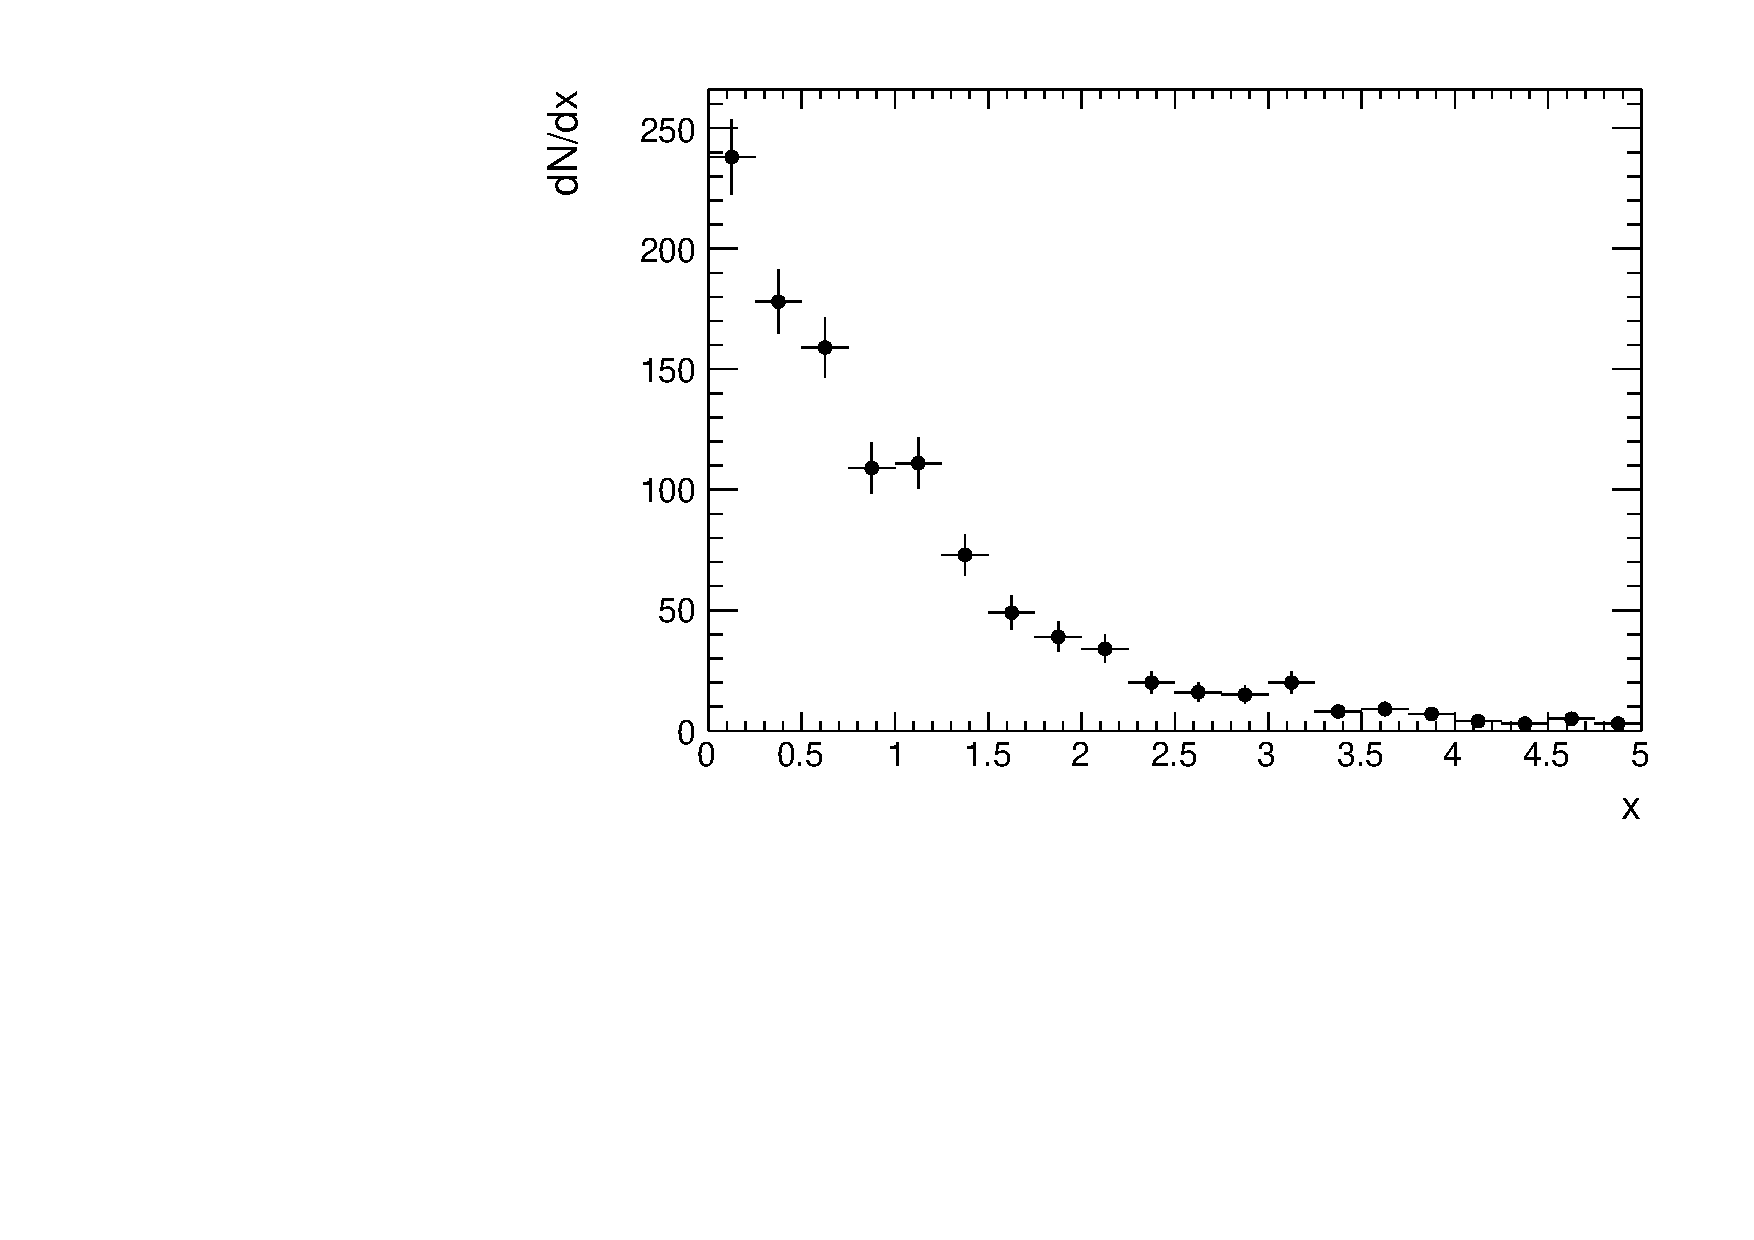
\includegraphics[width=0.45\textwidth]{randomvar.pdf}\hfill
%  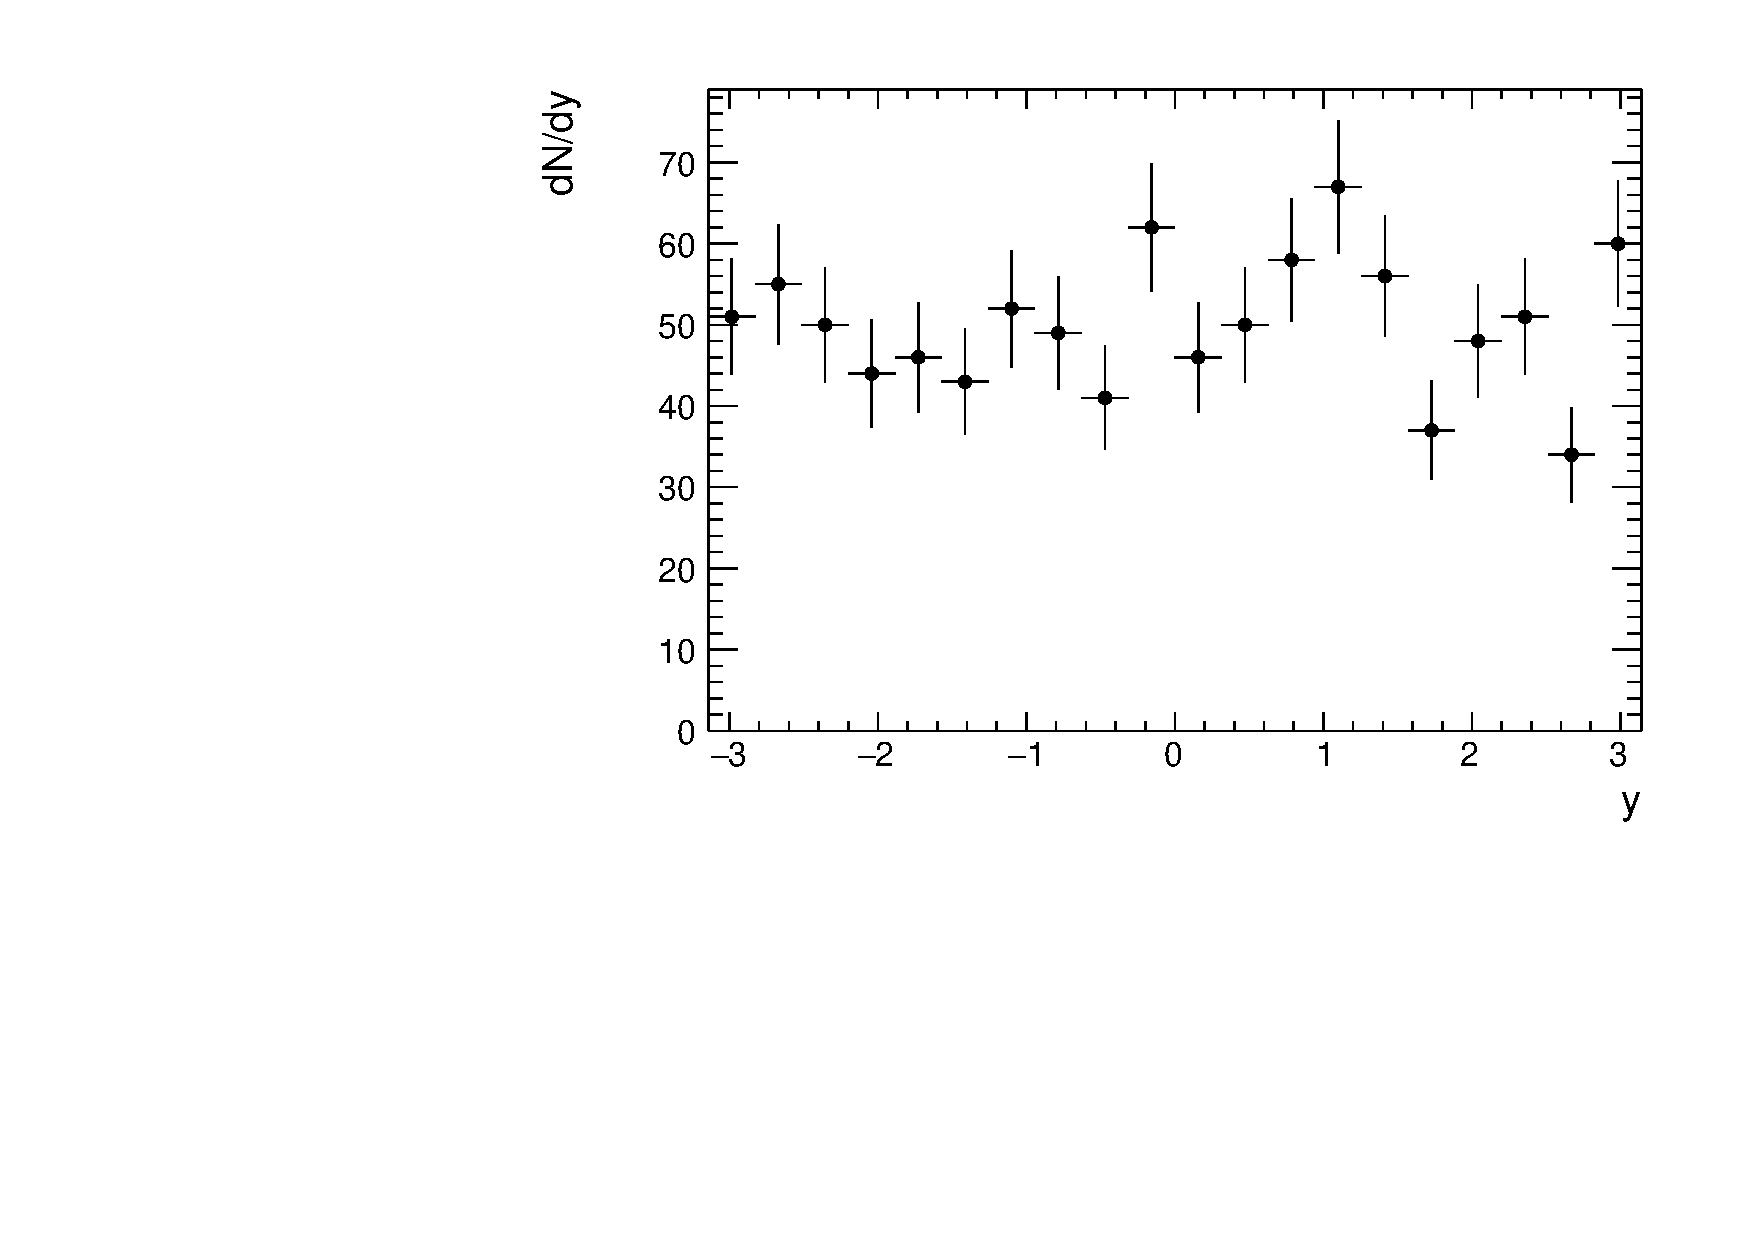
\includegraphics[width=0.32\textwidth]{randomvar2.pdf}\hfill
 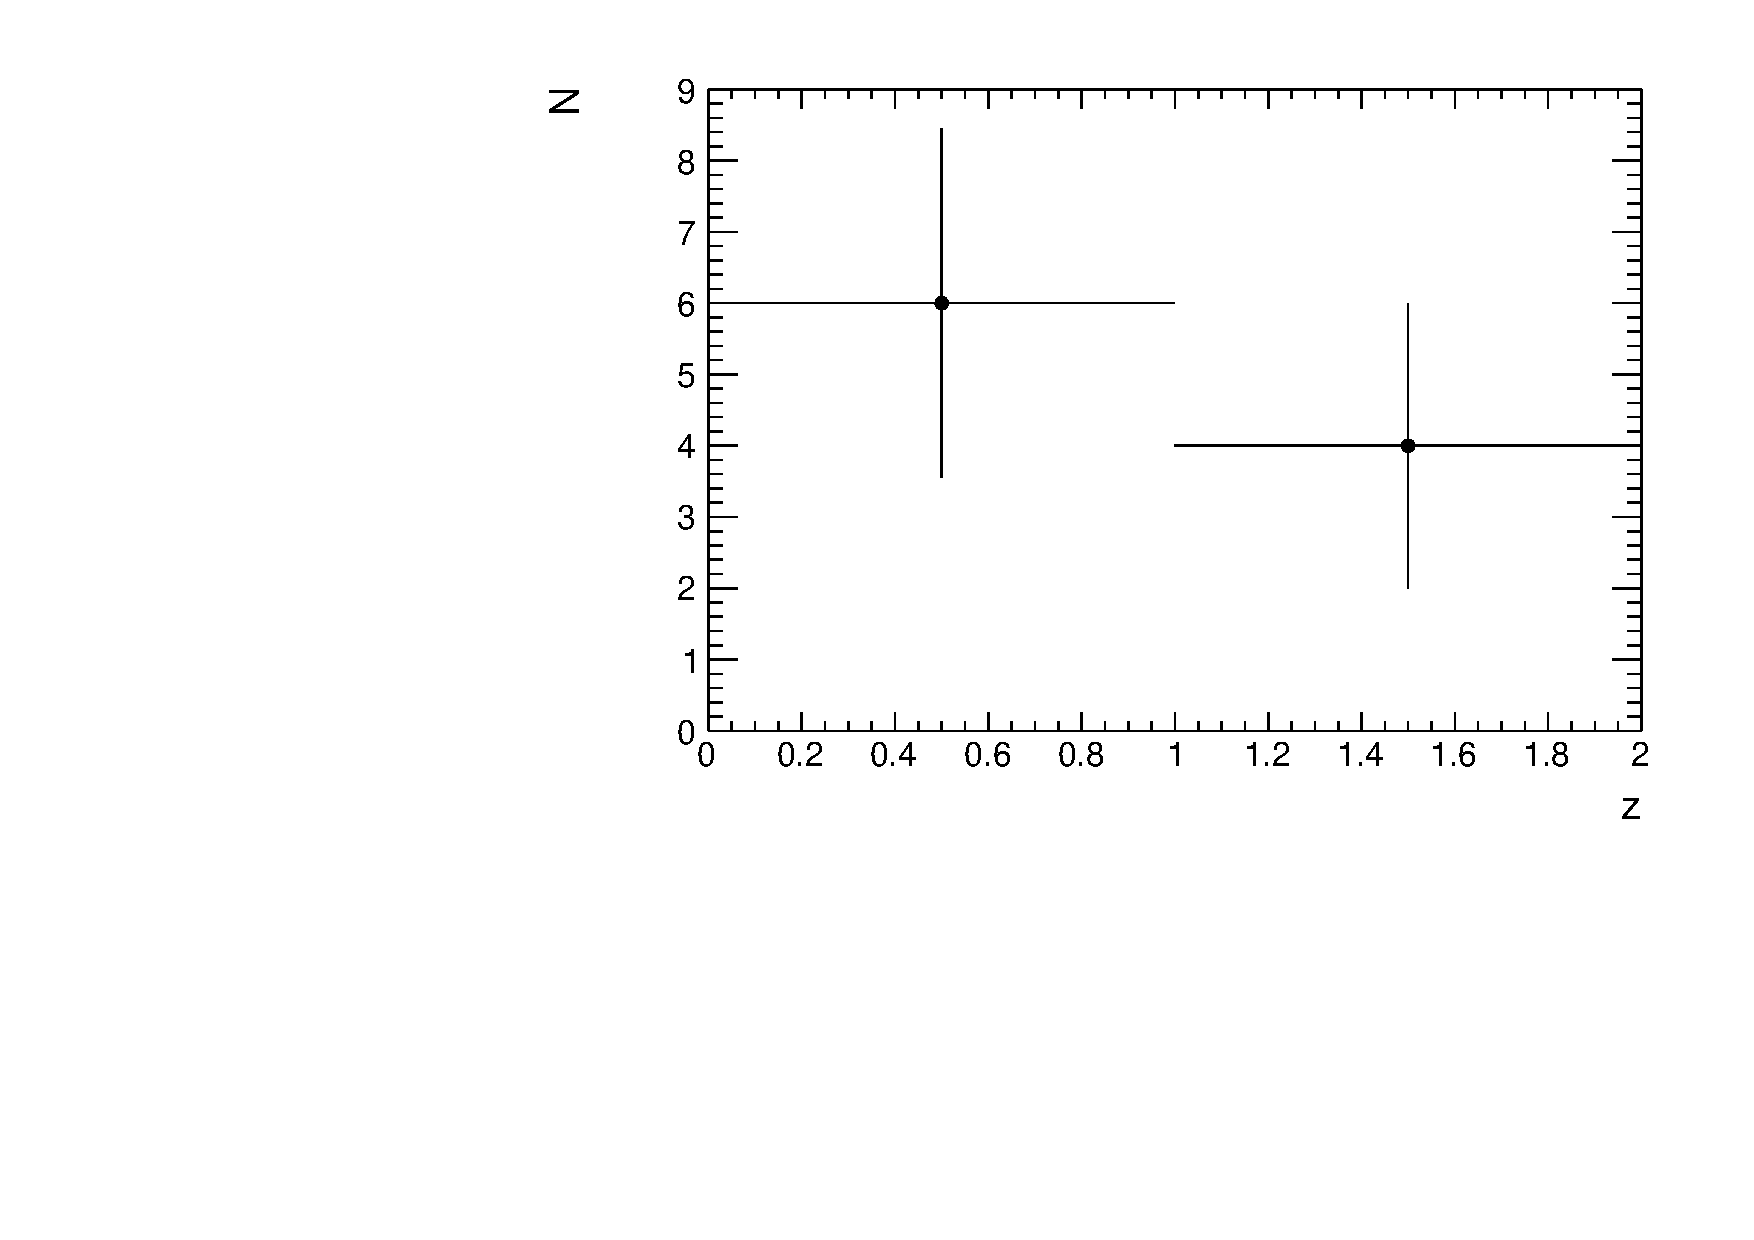
\includegraphics[width=0.45\textwidth]{randomvar3.pdf}
 
 \begin{block}{Random variable: definition}
  A random variable is a variable whose possible values are outcomes of a random phenomenon. It usually denoted with a capital letter (e.g. $X$).
  
  The ensemble of the exclusive possible numerical values of $X$ is the sample space $\Omega$:
  
  $$\Omega = \left\{ x_1, x_2, \dots \right\}$$
 \end{block}
 
 Examples:
 
 \begin{itemize}
  \item $x$: \only<2>{lifetime of a particle? $\Omega = [0, +\infty [$}
%   \item $y$: \only<2>{measurement of the azimuthal angle?}
  \item $z$: \only<2>{tossing of a coin? (heads = 0, tails = 1) $\Omega = \{0,1\}$}
 \end{itemize}
\end{frame}

\begin{frame}
 \frametitle{Mathematical probability}
 
 \begin{block}{Definition}
  Given a random variable $X$ and a sample space $\Omega$, a function $P$ is a probability if it obeys the \textbf{Kolmogorov axioms}:
  
  \begin{enumerate}
   \item<1-> $\forall x \in \Omega, P(x) \geq 0$ (and $P(x) \in \mathbb{R})$
   \item<2-> $\forall A, B \subset \Omega / A \cap B = \emptyset, P(A \cup B) = P(A) + P(B) $
   \item<3-> $P(\Omega) = 1, P(\emptyset)=0$ 
  \end{enumerate}

 \end{block}
 
 \uncover<4>{
 In other words, in the discrete case $\Omega = \{ x_i \}$
 
 \begin{enumerate}
  \item $P(x_i \geq 0$ for all $i$
  \item $P(x_i \text{ or } x_j) = P(x_i) + P(x_j)$
  \item $\sum_\Omega P(x_i) = 1$
 \end{enumerate}
}

\end{frame}

\begin{frame}
 \frametitle{Frequentist probability}
 
 \begin{block}{Definition}
 Frequentist probability is defined in an empiric way. Given a random variable $X$ and a sample space $\Omega$, we repeat the experiment $N$ times and measure the outcome of $X$.
 
 For $A \subset \Omega$, and if we measure $n$ times $X \in A$, we then define 
 
 $$P(A) = \lim_{N \to \infty} \frac{n}{N}$$
\end{block}

\begin{itemize}
 \item Important implication: frequentist probability can only be applied to repeatable experiments. The frequentist probability that it rains tomorrow cannot be defined!
 \item In particular: $P(\text{constant of nature} \in \text{(some interval)})$ or $P(\text{SUSY is true})$ \alert{do not exist} (in a usueful way) for this definition of $P$ (at least in one universe).
\end{itemize}

\end{frame}

\begin{frame}
 \frametitle{Bayesian probability}
 
 \begin{block}{definition}
  Bayesian probability is subjective and can be for instance defined using the \emph{degree of belief} (Finetti), with the notion of \emph{coherent bet}:
  
  $$P(A) = \frac{\text{money that you are ready to bet on measuring } X \in A}{\text{money that you stand to win}}$$
 \end{block}
 
 \begin{itemize}
  \item Bayesian is as much a property of the observer as of the system being observed.
  \item It depends on the state of the observer's knowledge, and will in general change as the observer obtains more knowledge.
  \item $P(\text{constant of nature} \in \text{(some interval)})$ or $P(\text{SUSY is true})$ exist for you!
  \item Shown to be basis for coherent personal decision making.
 \end{itemize}


\end{frame}

\begin{frame}
 \frametitle{Properties of probabitilies}
 
 \begin{block}{Addition law}
  Given $A, B \subset \Omega$, 
  
  $$P(A \cup B) = P(A) + P(B) - P(A \cap B)$$
 \end{block}
 
 \uncover<2->{\begin{block}{Conditional probability and independence}
 \begin{itemize}
  \item<2-> We define the conditional probability of $A$ given $B$ (i.e. of $x \in A$, given that already $x \in B$), written $P(A|B)$. Then:
  
  $$P(A \cup B) = P(A|B) P(B) = P(B|A) P(A)$$  
  
  \item<3> Sets $A$ and $B$ are said to be \emph{independent} if $$P(A|B) = P(A)$$ and equivalently $$P(A \cup B) = P(A) P(B)$$
 \end{itemize}
 \end{block}}


\end{frame}

\begin{frame}
 \frametitle{Graphical illustration and ``derivation'' of Bayes' Theorem}
 \vspace{-5pt}
 
 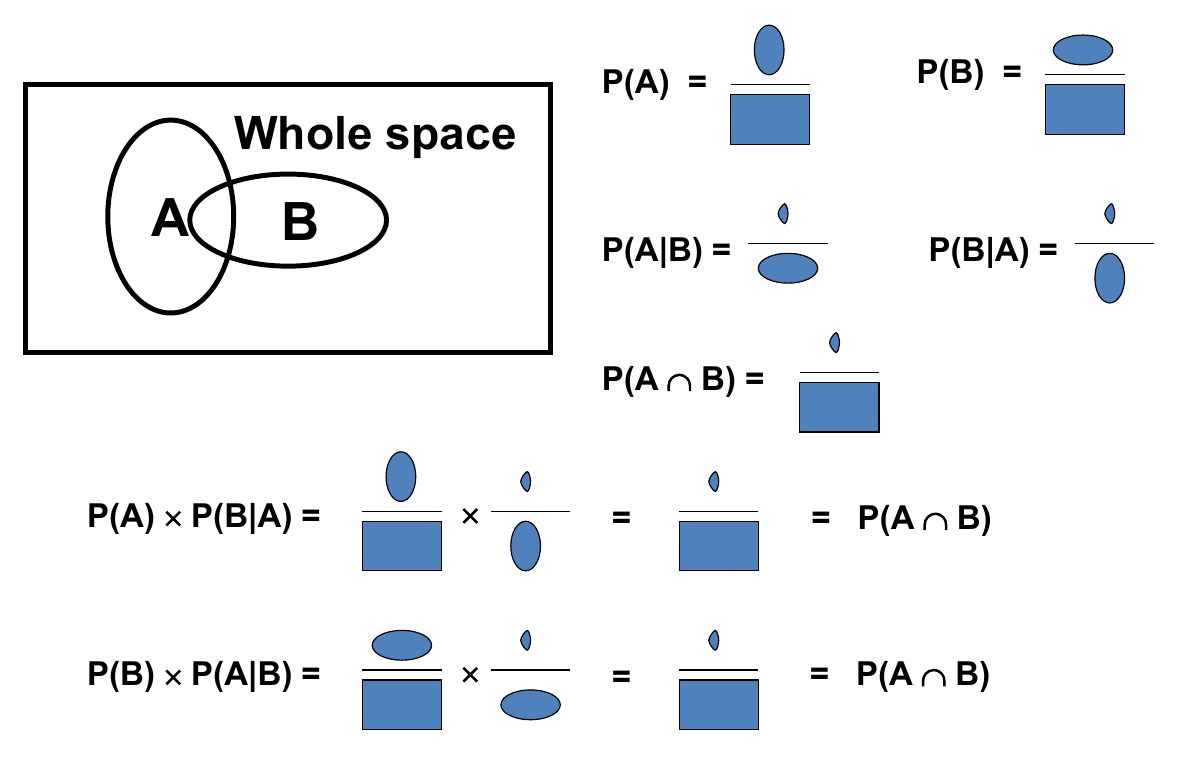
\includegraphics[width=\textwidth]{BayesTheorem.png}
 
 \begin{large}$$\alert{P(B|A) = \frac{P(A|B) P(B)}{P(A)}}$$                                              \end{large}
\end{frame}

\begin{frame}
 \frametitle{Bayesian interpretation}
 
 $A$ is theory, $B$ is experiment
 
 $$P(\text{theory} | \text{experiment}) = \frac{P(\text{experiment}|\text{theory}) P(\text{theory})}{P(\text{experiment})}$$
 
 \begin{itemize}
  \item $P(\text{theory} | \text{experiment})$ is called the \textbf{posterior probability}.
  \item $P(\text{theory})$ is called the \textbf{prior probability}.
 \end{itemize}

\end{frame}


\begin{frame}
 \frametitle{Example of Bayes' theorem using frequentist probability}
 
 A b-tagging method is developed and one measures:
 
 \begin{itemize}
  \item $P(\text{btag} | \text{b-jet})$, i.e., efficiency for tagging b’s
  \item $P(\text{btag} | \text{not a b-jet})$, i.e., efficiency for background
  \item $P(\text{no btag} | \text{b-jet}) = 1 - P(\text{btag} | \text{b-jet})$
  \item $P(\text{no btag} | \text{not a b-jet}) = 1 - P(\text{btag} | \text{not a b-jet})$
 \end{itemize}
 
 \vspace{10pt}
 
Question: Given a selection of jets tagged as b-jets, what
fraction of them is b-jets? I.e., what is $P(\text{b-jet} | \text{btag})$ ?

\vspace{10pt}

\uncover<2>{
Answer: Cannot be determined from the given information!

Need in addition: $P(\text{b-jet})$, the true fraction of all jets that are
b-jets. Then Bayes’ theorem inverts the conditionality:

$$P(\text{b-jet} | \text{btag}) \propto P(\text{btag} |\text{b-jet}) P(\text{b-jet})$$
}

\end{frame}
\begin{frame}
 \frametitle{Example of Bayes' theorem using frequentist probability}
 
 In HEP, as noted, $P(\text{btag} | \text{b-jet})$ is called the \emph{efficiency} for tagging b’s.
 
 Meanwhile $P(\text{b-jet} | \text{btag})$ is often called the \emph{purity} of a sample of b-tagged jets.
 
As this is a pretty ``easy'' distinction, it is helpful to keep it in mind when one encounters cases where it is perhaps tempting to make the logical error of equating $P(A|B)$ and $P(B|A)$.

\end{frame}

\begin{frame}
 \frametitle{Example  of Bayes' theorem using Bayesian probability}
 
 In a background-free experiment, a theorist uses a ``model'' to
predict a signal with Poisson mean of 3 events. From Poisson
formula we know:

\begin{itemize}
 \item $P(\text{0 events} | \text{model true}) = 3^0 e^{-3}/0! = 0.05$
 \item $P(\text{0 events} | \text{model false}) = 1.0$
 \item $P(>\text{0 events} | \text{model true}) = 0.95$
 \item $P(>\text{0 events} | \text{model false}) = 0.0$
\end{itemize}

The experiment is performed and \emph{zero events are observed}.

\vspace{10pt}

Question: Given the result of the expt, what is the probability that
the model is true? I.e., What is $P(\text{model true} | \text{0 events})$ ?

\vspace{10pt}

\uncover<2>{Answer: Cannot be determined from the given information!

Need in addition: $P(\text{model true})$, the degree of belief in the
model prior to the experiment. Then Bayes’ theorem inverts the
conditionality:

$$P(\text{model true} | \text{0 events}) \propto P(\text{0 events} | \text{model true}) P(\text{model true})$$

or in other words (using Bayes' theorem with $A = \text{0 events}$, $B = \text{model true}$):

$$P(\text{model true} | \text{0 events}) = \frac{0.05  P(\text{model true})}{1 - 0.95 P(\text{model true})}$$
}

\end{frame}

\begin{frame}
 \frametitle{Example  of Bayes' theorem using Bayesian probability}
 
 $$P(\text{model true} | \text{0 events}) = \frac{0.05  P(\text{model true})}{1 - 0.95 P(\text{model true})}$$
 
Limiting cases to lowest order in $\epsilon$, with $\epsilon \ll 1$:

\vspace{10pt}

Let ``model'' be the Standard Model of particle physics, prior $P(\text{model true}) = 1 - \epsilon$, then $P(\text{model true} | \text{0 events}) \approx 1 - 20\epsilon$

Still very high degree of belief! Tempting mistake: ``$P(\text{0 events} | \text{model true}) = 5\%$, and 0 events observed, means there is 5\% chance the S.M. is true'' (UGH!)

\vspace{10pt}

Let ``model'' be large extra dimensions, prior $P(\text{model true}) = \epsilon$, then $P(\text{model true} | \text{0 events}) \approx 0.05 \epsilon$

Low prior belief becomes even lower.

\vspace{10pt}

N.B. More realistic examples are of course more complex.

\end{frame}

\begin{frame}
 \frametitle{Note relative to decisions}
 
 Suppose that as a result of the previous experiment, your degree
of belief in the model is $P(\text{model true} | \text{0 events}) = 99\%$, and you
need to decide on an action (making a press release, or planning
next experiment), based on the model being true.
Question: What should you decide?

\vspace{10pt}

\uncover<2>{Answer: Cannot be determined from the given information!

\vspace{10pt}

Need in addition:
The \emph{utility} function (or its negative, the \emph{loss} function), which
quantifies the relative costs (to You) of

\begin{itemize}
 \item Type I error (declaring model false when it is true), and
 \item Type II error (not declaring model false when it is false).
\end{itemize}
}

\end{frame}

\begin{frame}
\frametitle{Note relative to decisions}

Thus, Your decision, requires two subjective inputs: Your prior
probabilities, and the relative costs to You of outcomes.
Statisticians often focus on decision-making.

In HEP, the tradition thus far is to communicate experimental
results (well) short of formal decision calculations.

It will become clear when we come to hypothesis testing: 

Frequentist (classical) ``hypothesis testing'' (especially with
conventions like 95\% C.L. or $5\sigma$ ) is not a complete theory of
decision-making!

It is important to keep this in mind, since the ``accept/reject''
language of classical hypothesis testing is too
simplistic for ``deciding'' in important situations.

\end{frame}


\begin{frame}
 \frametitle{Discrete random variables $X$}
 
 
  $X \in \Omega = \{ x_1, x_2, \dots, x_N \}$ (where $N \in \mathbb{N} \cup \{+\infty\}$)
  
  Then, if $p_i = P(x_i)$:
  
  \begin{itemize}
   \item $\forall i, p_i \in [0,1]$
   \item $\sum_{i=1}^N p_i = 1$
  \end{itemize}

 \end{frame}
 
 \begin{frame}
 \frametitle{Continuous random variables $X$}
 
 \begin{block}{Cumulative function}
  $X \in \Omega = [a,b]$ where $(a,b) \in (\mathbb{R} \cup \{-\infty,+\infty\})^2$
  
  The probability law is defined using a function $F(x_0) = P(x \leq x_0)$, called the \alert{cumulative function}.
 \end{block}
 
 The cumulative function is such that:
 
 \begin{itemize}
  \item $F(b) = 1$
  \item $F(a) = 0$
  \item $\forall x \in [a,b], \frac{\dd F}{\dd x}(x) \geq 0$
 \end{itemize}

 \begin{block}{Probability density function (pdf)}
  The probability density function is defined as:
  
  $$f(x) \dd x = F(x+\dd x) - F(x) = P(X \in [x, x+\dd x])$$
  
  or, in other words:
  
  $$f(x) = \frac{\dd F}{\dd x}(x)$$
 \end{block}



\end{frame}

\begin{frame}
 \frametitle{Multi-dimensional variable}
 
 Example: $X = (x,y,z)$. 
 Then $P(x \in [x_0, x_0 + \dd x], y \in [y_0, y_0 + \dd y], z \in [z_0, z_0 + \dd z]) = f(x_0,y_0,z_0) \dd x \dd y \dd z$ where $f$ is the pdf.
 
 \begin{block}{Definition: marginal pdf}
  $$f_X (x) = \int \dd y^\prime \dd z^\prime\, f(x,y^\prime,z^\prime)$$
  
  $f_X$ is a \textbf{projection} of $f$
 \end{block}
 
 \begin{block}{Definition: conditional pdf}
  $$f_C (x, y_0, z_0) = \frac{f(x,y_0,z_0)}{\int \dd x^\prime f(x^\prime, y_0, z_0)}$$
  
  $f_C$ is a \textbf{``section''} of $f$
 \end{block}

 \begin{block}{Definition: independent variables}
  Given two random variables $X$ and $Y$, \\
  $X$ and $Y$ are independent iff $f(x,y) = f_X(x) f_Y(y)$.
 \end{block}


 
\end{frame}

\begin{frame}
 \frametitle{Change of variable}
 
 Let $f(\vec{x})$ be a pdf and a change of variables $h: \vec{x} \mapsto \vec{y} = h(\vec{x})$, $[\vec{x}, \vec{x} + \dd\vec{x}] \to [\vec{y}, \vec{y} + \dd\vec{y}]$
 
 \vspace{10pt}
 
 \structure{What is the pdf of $\vec{y}$: $g(\vec{y})$?}
 
 \uncover<2>{\only<2>{
 \begin{block}{If $x$ and $y$ are scalars, and $h$ bijective}
  \begin{eqnarray}
   g(y) \dd y & = & f(x) \dd x \nonumber \\
   g(y) & = & f(x) \left| \frac{\dd x}{\dd y}\right| = \frac{f(x)}{|h^\prime (x)|} \nonumber \\
   \structure{g(y)} & \structure{=} & \structure{\frac{f(x)}{\left| \frac{\dd y}{\dd x} \right|}}   
  \end{eqnarray}
  
  NB: $g$ is not defined where $h^\prime(x) = 0$.

 \end{block}

 }}
 
 \only<3>{
 \begin{block}{If $x$ and $y$ are scalars, and $h$ bijective}
  Several $[x_i,x_i+\dd x]$ correspond to a given $[y,y+\dd y]$
  
  Then \structure{$$g(y) = \sum{i, h(x_i) = y} \frac{f(x_i)}{|h^\prime(x_i)|}$$}
 \end{block}
 
 Examples:
 
 \begin{itemize}
  \item $$y = h(x) = x^2\quad \longrightarrow \quad g(y) = \frac{f(\sqrt{y}) + f(-\sqrt{y})}{2\sqrt{y}}$$
  \item $$y = h(x) = |x|\quad \longrightarrow \quad g(y) = \frac{f(y) + f(-y)}{1}$$
 \end{itemize}


 }
 
 \only<4>{
 \begin{block}{Case of multiple dimensions and a bijective $h$}
  \structure{$$g(\vec{y}) = \frac{f(\vec{x})}{\left| \det \left( \frac{\partial \vec{h}}{\partial \vec{x}} \right) \right|}$$}
  
  The denominator is the jacobian of the transformation.
 \end{block}

 }
 
\end{frame}

\section{Properties of pdfs}

\begin{frame}
 \frametitle{Properties of pdfs}
 
 $$X,\qquad f(x),\qquad x \in \Omega$$
  
\end{frame}

\begin{frame}
 \frametitle{Properties of pdfs}
 
 \begin{block}{Expectation of a function, $g(X)$}
  
  $$E(g) = \int_\Omega g(X) f(X) \dd X$$
  
  {\footnotesize NB: in the discrete case, $\int \leftarrow \sum$, $f(x) \dd x \leftarrow p_i (x_i)$ }
 \end{block}
 
 \begin{block}{Mean $\mu$ ($= \bar{X} = \langle X \rangle$)}
 
  $$\mu = E(X) = \int X f(X) \dd X$$
 \end{block}
 
 \end{frame}

\begin{frame}
 \frametitle{Properties of pdfs}

 \begin{block}{Variance $V$, standard deviation $\sigma$}
  \begin{eqnarray}
   V = \sigma^2 & \equiv & E \left( (X-\mu)^2 \right) \nonumber\\
   & = & E \left( X^2 - 2 \mu X + \mu^2\right) \nonumber\\
   \structure{V} & \structure{=} & \structure{E\left( x^2 \right) - \mu^2} \nonumber
  \end{eqnarray}

 \end{block}

 NB: not always defined (e.g. for the Breit-Wigner, aka Cauchy, distribution: undefined mean, infinite variance).

\end{frame}

\begin{frame}
 \frametitle{Moments}
 
 \begin{block}{Definition}
  \begin{itemize}
   \item Central moment: $E\left[ (X-\mu)^n \right]$
   \item Algebaric moment: $E\left[ X^n \right]$
  \end{itemize}

 \end{block}

 Particular cases: 
 
 \begin{itemize}
  \item $n=3$ central moment: \structure{skewness}. Measures the left-right asymmetry of the pdf.
  \item $n=4$ central moment: \structure{kurtosis}. Measures the size of the tails of the distribution (if positive, then larger tails than a Gaussian).
 \end{itemize}

 
\end{frame}

\begin{frame}
 \frametitle{Characteristic function of a pdf}
 
 \begin{block}{Definition}
  \begin{eqnarray}
   \Phi_X (t) & \equiv & E(e^{itx}) \qquad t \in \mathbb{R} \nonumber \\
   & = & \int_\Omega e^{itx} f(x) \dd x \qquad \text{(continuous)}\nonumber \\
   & = & \sum_k p_k e^{i t x_k}\qquad \text{(discrete)} \nonumber 
  \end{eqnarray}

 \end{block}
 
 If the pdf is continuous, then 
 $$f(x) = \frac{1}{2 \pi} \int_{-\infty}^{+\infty} \Phi_X(t) e^{-itx} \dd t$$
 
 Properties: $\Phi_X (0) = 0$, $|\Phi_X(t)| \leq 1 \quad \forall t$
 
 For $X,Y$ two independent variables: $\Phi_{X+Y}(t) = \Phi_X(t) \Phi_Y(t)$


\end{frame}

\begin{frame}
 \frametitle{Taylor development of the characteristic function}
 
 \begin{block}{}
  $$\Phi_X(t) = E(e^{itX}) = E \left( \sum_{n=0}^{+\infty} \frac{(itX)^p}{n!} \right) = \sum_{n=0}^{+\infty} \frac{(it)^n}{n!} E(X^n) $$
  
  where $E(X^n)$ is the $n$\ith moment
 \end{block}
 
 % I skip here a discussion from the ED class

\end{frame}

\begin{frame}
 \frametitle{Case of several variables}
 
 \begin{block}{Covariance $C(X,Y)$}
  $$C(X,Y) \equiv E \left( (X-\mu_X) (Y-\mu_Y) \right) = E(XY) - E(X) E(Y)$$
 \end{block}
 
 \begin{block}{Correlation coeffcient (or Pearson coefficient)}
  $$\rho(X,Y) \equiv \frac{C(X,Y)}{\sigma_X \sigma_Y}$$
 \end{block}
 
 \begin{block}{Schwartz lemma}
  $|\rho(X,Y)| \leq 1$
 \end{block}

 Demo of the Schwartz lemma:
 
 $$\forall \alpha, V(\alpha X + Y) = \alpha^2 V(X) + V(Y) + 2 \alpha C(X,Y) \geq 0$$
 
 This quadratic form can have one solution at most, hence its determinant is $\leq 0$: 
 
 $$C(X,Y)^2 - V(X) V(Y) \leq 0 \quad \text{(QED)}$$ 


\end{frame}

\begin{frame}
 \frametitle{Covariance: special cases}
 
 \begin{block}{Independent variables}
  $$X,Y \text{ independent} \Rightarrow C(X,Y) =0, \rho(X,Y) = 0$$
  
  NB: the opposite is not true (can have $C(X,Y)=0$ but $X$ and $Y$ not independent).
 \end{block}
 
 \begin{columns}
  \begin{column}{0.27\textwidth}
   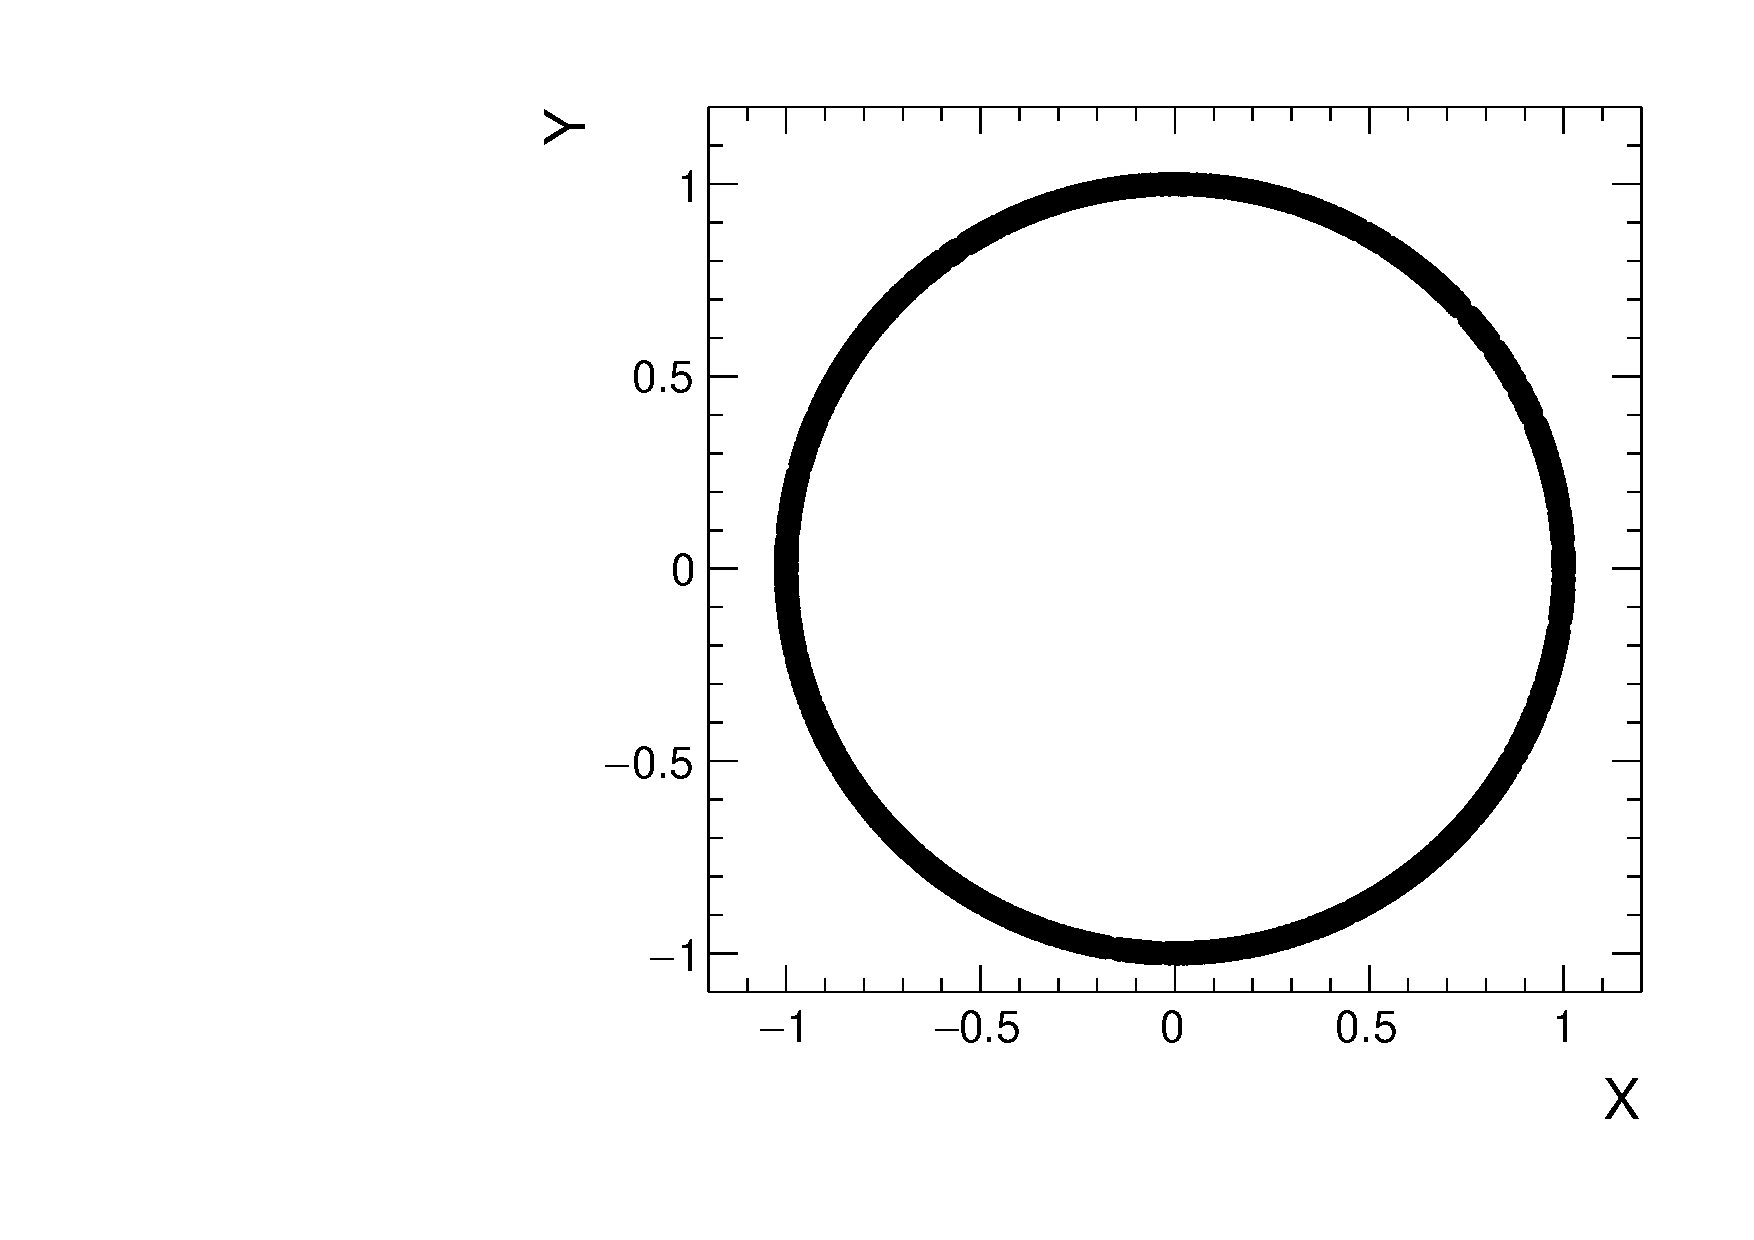
\includegraphics[width=\textwidth]{circle}

   \centering
   $\rho=0$,\\ not independent
  \end{column}
  \begin{column}{0.27\textwidth}
   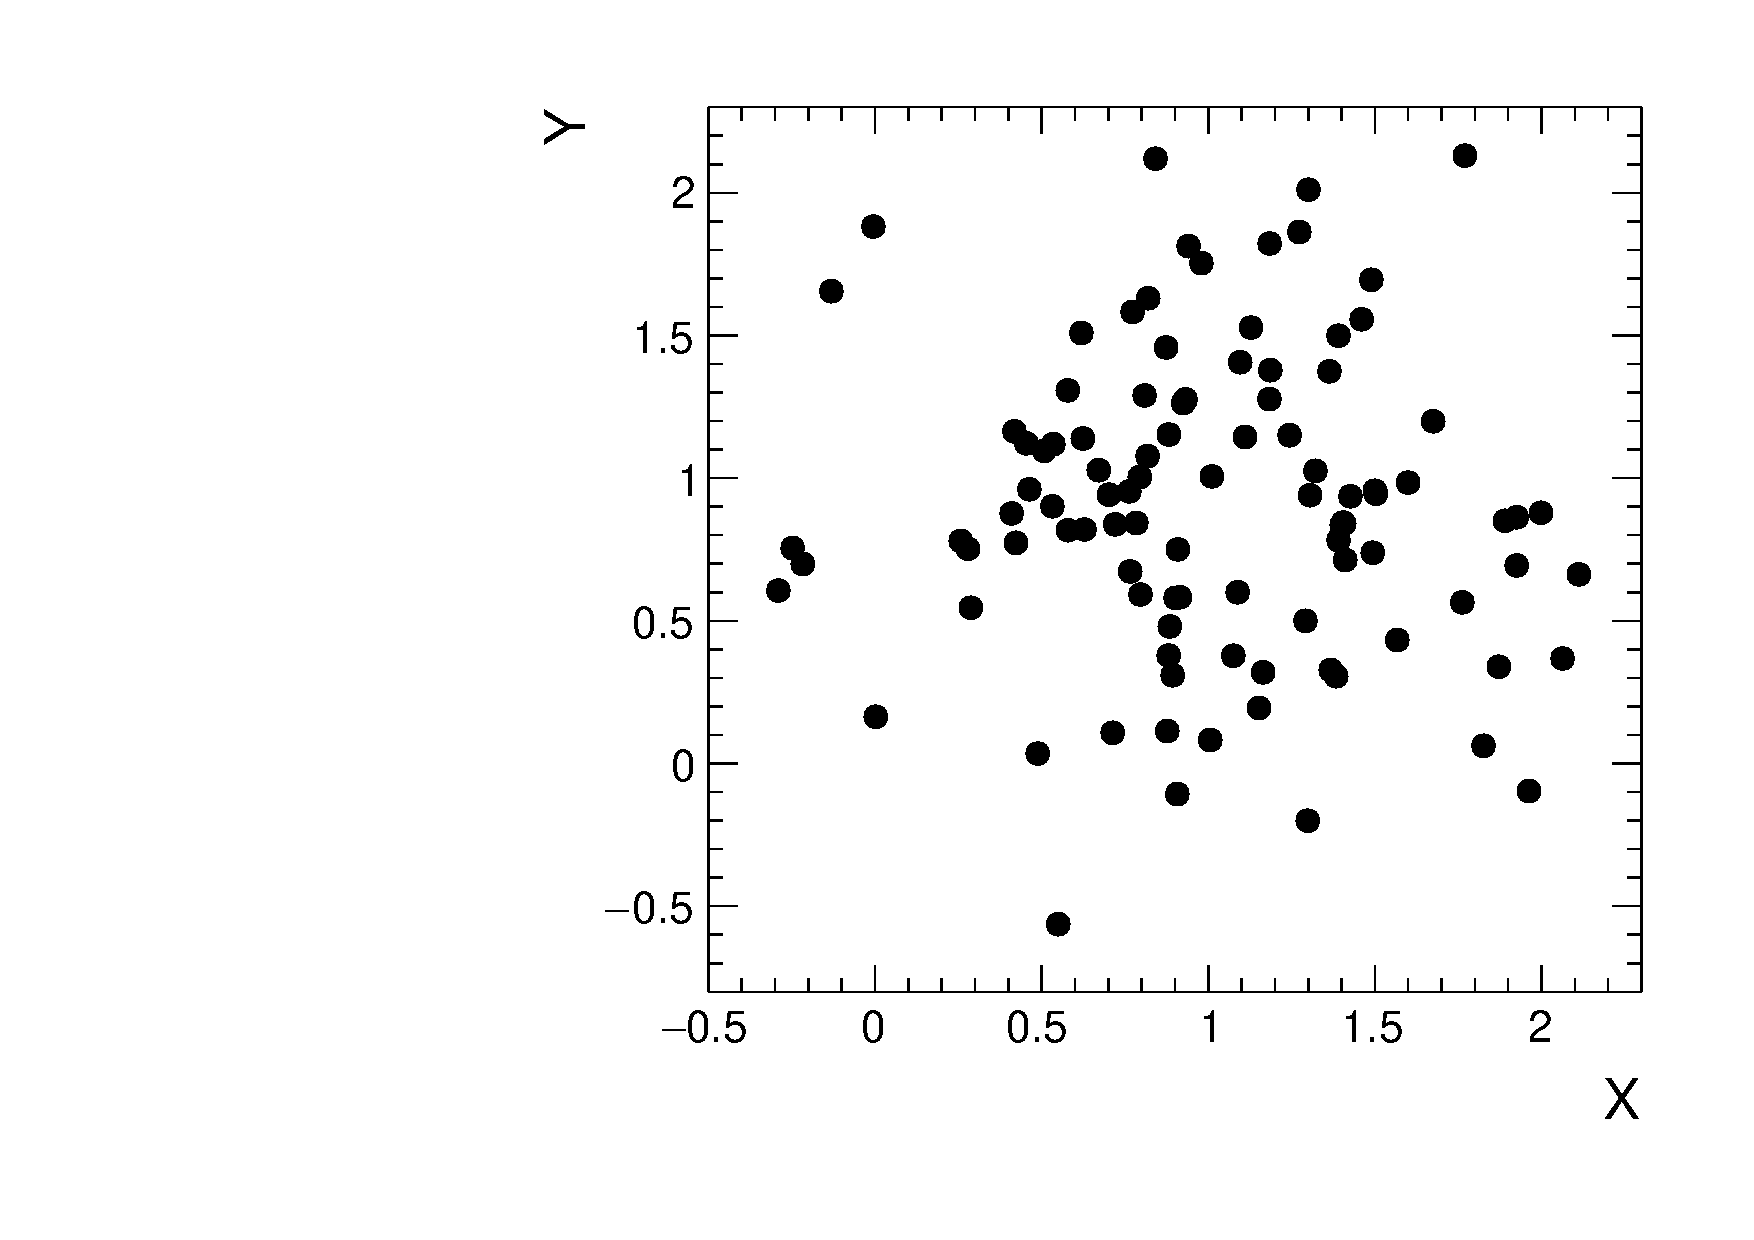
\includegraphics[width=\textwidth]{uncor}
   
   \centering
   $\rho=0$,\\ independent
  \end{column}
  \begin{column}{0.27\textwidth}
   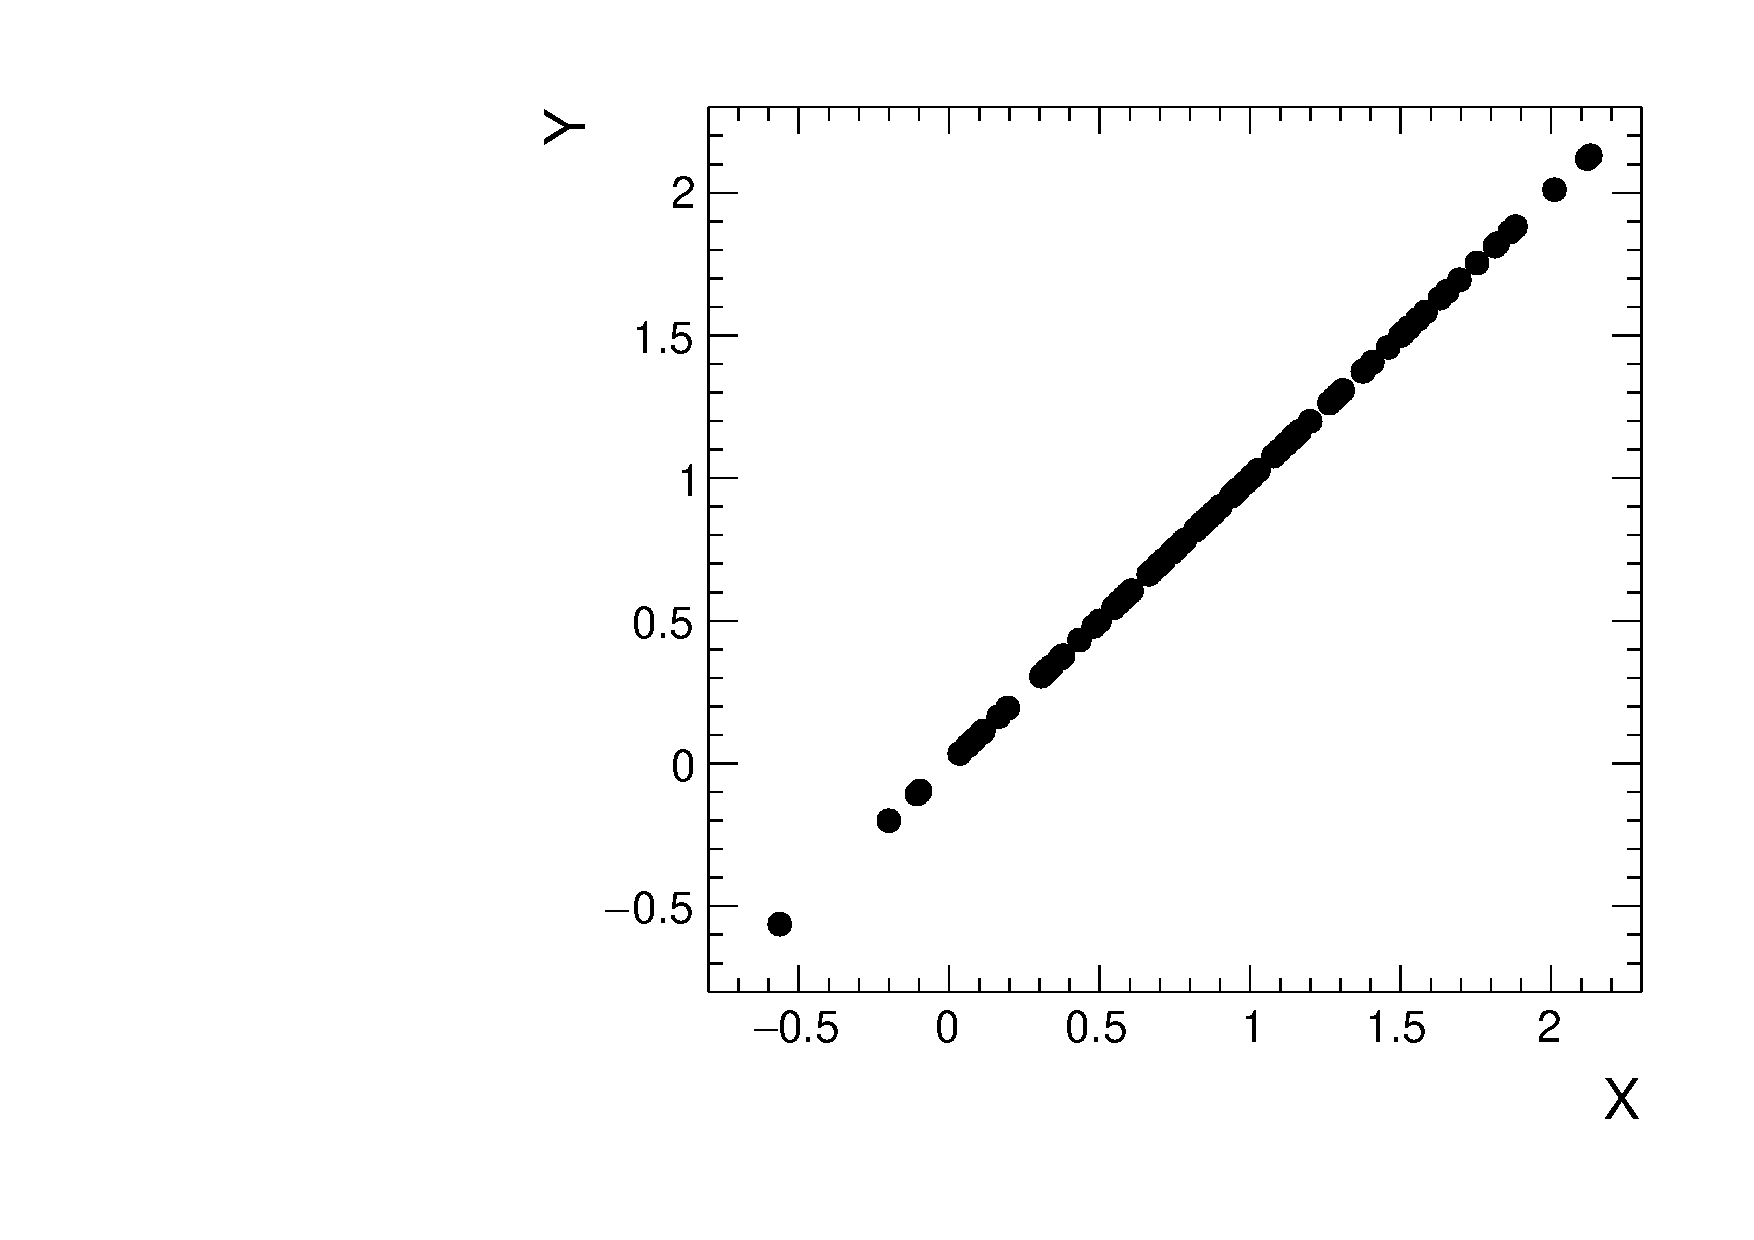
\includegraphics[width=\textwidth]{cor}
   
   \centering
   $\rho=1$,\\ complete correlation
  \end{column}
  \begin{column}{0.27\textwidth}
   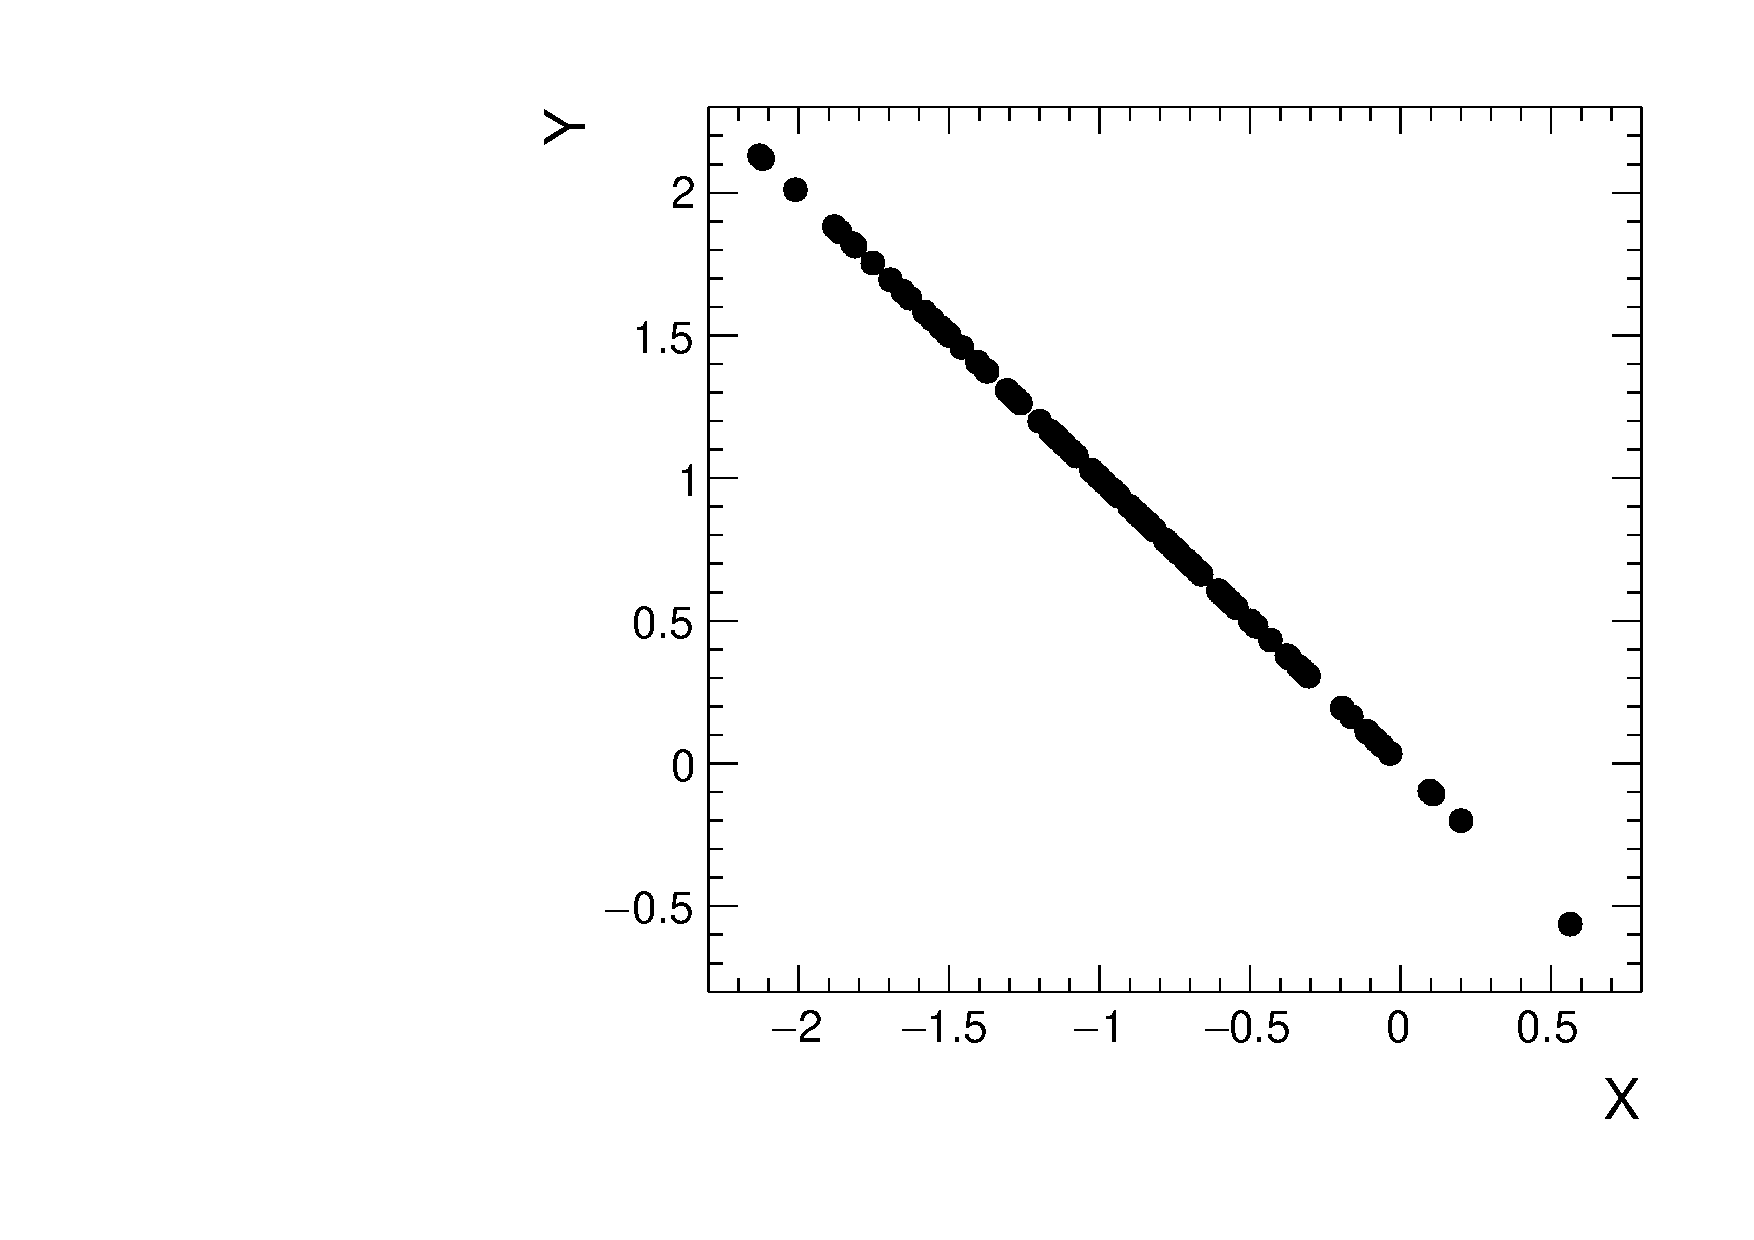
\includegraphics[width=\textwidth]{anticor}
   
   \centering
   $\rho=-1$,\\ complete anti-correlation
  \end{column}
 \end{columns}


\end{frame}

\begin{frame}
 \frametitle{Covariance matrix}
 
 \begin{block}{}
  $$\vec{X} = (X_1, \dots, X_N)$$
  
  $$V_{\vec{X}} = \begin{pmatrix}
                   \sigma_1^2 & C(X_1,X_2) & \cdots & C(X_1,X_N) \\
                   C(X_1,X_2) & \sigma_2^2 & \cdots & C(X_2,X_N) \\
                   \vdots & \ddots & \ddots &  \vdots \\
                   \vdots & \ddots & \ddots &  \sigma_N^2
                   \end{pmatrix}
$$
 \end{block}
 
 \begin{block}{Properties}
  \begin{itemize}
   \item The covariance matrix is symmetric.
   \item All its eigen values are positive.
  \end{itemize}

 \end{block}

\end{frame}

\begin{frame}
 \frametitle{Covariance matrix: change of variables}
 
 \begin{block}{Linear change of variables $\vec{Z} = A \vec{X} + B$}
  $$V_{\vec{Z}} = A\, V_{\vec{X}}\, ^t A$$
 \end{block}
 
 \begin{block}{}
  $$E \left( \sum_{i=1}^{N} a_i X_i \right) = \sum_{i=1}^{N} a_i E(X_i)$$
  $$V \left( \sum_{i=1}^{N} a_i X_i \right) = \sum_{i=1}^{N} a_i V(X_i) + 2 \sum_{i=1}^{N-1} \sum_{j=i+1}^{N} a_i a_j C(X_i,X_j)$$
 \end{block}

 \begin{block}{Nonlinear change of variables $\vec{Y} = \vec{H} (\vec{X})$}
  There is no exact formula for $V_{\vec{Y}}$. However,
  
  $$V_{\vec{Y}} = D V_{\vec{X}} D^{-1}$$
  
  where $D$ is the matrix of the derivatives (which determinant is the Jacobian), evaluated in $\vec{X}_0 = E(\vec{X})$.
 \end{block}


\end{frame}

\begin{frame}
 \frametitle{Application: sample mean}
 
 
 
  Assume $N$ realisations of $X$ for $N$ independent trials. For each trial, we have a pdf $f(x)$ with mean $\mu$ and variance $\sigma^2$. 
  
  Define $\bar{X} = \frac{1}{N} \sum_{i=1}^{N} X_i$
  
  \begin{itemize}
   \item $E(\bar{X}) = \frac{1}{N} \sum_i E(X_i) = \frac{1}{N} N \mu = \mu$ 
   \item $V(\bar{X}) = \frac{\sigma^2}{N}$
  \end{itemize}
 

\end{frame}

\section{Discrete laws}

\begin{frame}
 \frametitle{Outline}
 
 \tableofcontents[current]
\end{frame}

\begin{frame}
 \frametitle{Binomial law}
 
 Let $X$ be a random variable, with $x \in \Omega$, and let $A \subset \Omega$, with $P(A) = p$
 
 We repeat the experiment $N$ times, and count $n$ the number of times that we got $x \in A$. $n$ is a random variable and follows a binomial law.
 
 \begin{block}{Binomial law}
  $$P(n) = B(n;N,p) = \left( ^N_n \right) p^n (1-p)^{N-n}$$
 \end{block}
 
 \begin{block}{Properties}
  \begin{itemize}
   \item Mean: $E(n) = pN$
   \item Variance: $V(n) = N p (1-p)$
  \end{itemize}
 \end{block}

\end{frame}

\begin{frame}
 \frametitle{Multinomial law}
 
 Let there be $K$ exclusive realisations: $Q_1, Q_2, \dots, Q_K$, with respective probabilities $p_1, p_2, \dots, p_K$ ($\sum_{i=1}^K p_i = 1$)
 
 We repeat the experiment $N$ times, and count $n_1$ in $Q_1$, $n_2$ in $Q_2$, \dots, $n_K$ in $Q_K$.
 
 \begin{block}{Multinomial law}
  $$P(n_1,n_2,\dots,n_K) = \frac{N!}{n_1! \dots n_K!} p_1^{n_1} \dots p_K^{n_K} = \frac{N!}{\prod_{i=1}^{K} n_i!} \prod_{i=1}^K p_i^{n_i}$$
  
  Parameters: $N$, $\{p_i\}_{i=1..K}$
 \end{block}
 
 Example: histogram with $K$ bins and $N$ events ($N$ \textbf{fixed})

 \begin{block}{Properties}
  \begin{itemize}
   \item Covariance: $C(n_i,n_j) = -N p_i p_j$
   \item Correlation: $\rho (n_i,n_j) = \sqrt{\frac{p_i p_j}{(1-p_i)(1-p_j)}}$
  \end{itemize}
 \end{block}

\end{frame}

\begin{frame}
 \frametitle{Poisson law}
 
 Typical case: probability of observing $n$ events during $\Delta t$, knowing that events come with a rate $\mu$. 
 \structure{It is the limit of the binomial law, with $N \to \infty$, $p \to 0$, $Np = \mu$}
 
 \begin{block}{Poisson law}
  $$P_\mu(n) = \frac{\mu^n e^{-\mu}}{n!}$$
 \end{block}
 
 \begin{block}{Properties}
  \begin{itemize}
   \item Mean: $E(n) = \mu$
   \item Variance: $V(n) = \mu$ (and standard deviation $\sigma(n) = \sqrt{\mu}$)
  \end{itemize}
 \end{block}

 Example: radiactive sources, with $\nu$ counts per unit time. During an infinitesimal $\delta t$:
 
 \begin{itemize}
  \item $p(1) = \nu \delta t$ 
 \end{itemize}
 
 $$P(n) = \frac{(\nu t)^n e^{-\nu t}}{n!}$$


\end{frame}

\begin{frame}
 \frametitle{Sum of Poisson laws}
 
 Sum of independent Poisson laws:
 
 \begin{itemize}
  \item $N = n_1 + \dots + n_K$
  \item $P(n_1,\mu_1) \dots P(n_k,\mu_K)$
 \end{itemize}
 
 $$P(N) = P_{\mu = \mu_1 + \dots + \mu_K}(N)$$
 
 The sum of Poisson laws is a Poisson law which mean is the sum of the individual means.

\end{frame}

\section{Continuous laws}

\begin{frame}
 \frametitle{Outline}
 
 \tableofcontents[current]
\end{frame}

\begin{frame}
 \frametitle{Exponential law}
 
 \begin{block}{Exponential law}
  $f_\tau (t) = \frac{1}{\tau} e^{-t/\tau}$
 \end{block}
 
 Example: decay time of a particle
 
 \begin{block}{Properties}
  \begin{itemize}
   \item Mean: $E(t) = \tau$
   \item Variance: $V(t) = \tau$
  \end{itemize}

 \end{block}


\end{frame}

\begin{frame}
 \frametitle{Normal law (Gaussian)}
 
 \begin{block}{Normal law}
  $$f_{\mu,\sigma} (x) = \frac{1}{\sqrt{2\pi} \sigma} e^{-\frac{(x-\mu)^2}{2\sigma^2}}$$
 \end{block}
 
 \begin{block}{Properties}
  \begin{itemize}
   \item Mean: $E(x) = \mu$
   \item Variance: $V(x) = \sigma^2$
   \item All moments of order $>2$ are zero. In particular: skewness $=0$, kurtosis $=0$
  \end{itemize}
 \end{block}

 The cumulative function is called the error function: \structure{$F(x) = \text{erf}(x)$}

\end{frame}

\begin{frame}
 \frametitle{Normal law: some numbers}
 
 \begin{center}
  \begin{tabular}{c|c}
   FWHM\footnote{Full Width Half Maximum} & $\approx 2 \times 1.176 \sigma$ \\
   $P(-\sigma \leq x-\mu \leq \sigma$ & $\approx 0.68$ \\
   $P(-1.64 \sigma \leq x-\mu \leq 1.64 \sigma$ & 0.90 \\
   $P(-1.96 \sigma \leq x-\mu \leq 1.96 \sigma$ & 0.95 \\
   $P(-3.24 \sigma \leq x-\mu \leq 3.24 \sigma$ & 0.999 
  \end{tabular}

 \end{center}

\end{frame}

\begin{frame}
 \frametitle{Normal law of several variables}
 
 \begin{block}{Normal law of $K$ variables}
  $$f(\vec{X}) = \frac{1}{2\pi^{K/2} |\det V|^{1/2}} \exp \left( -\frac{1}{2} \left(\vec{X}-\vec{\mu}\right) V^{-1}  \left(\vec{X}-\vec{\mu}\right)^\text{T} \right)$$
  
  where $V$ is a positive definite matrix.
 \end{block}
 
 \begin{columns}
  \begin{column}{0.6\textwidth}
   
 
 \begin{block}{Properties}
  \begin{itemize}
   \item Mean: $E(\vec{X}) = \vec{\mu}$
   \item Covariance matrix: $C(\vec{X}) = V$
  \end{itemize}
 \end{block}
 
  \textbf{Careful!} 1D confidence intervals ($P(|X-\mu|<xx\sigma) = yy$) cannot be taken directly from the 1D case.
  \end{column}
  \begin{column}{0.4\textwidth}
   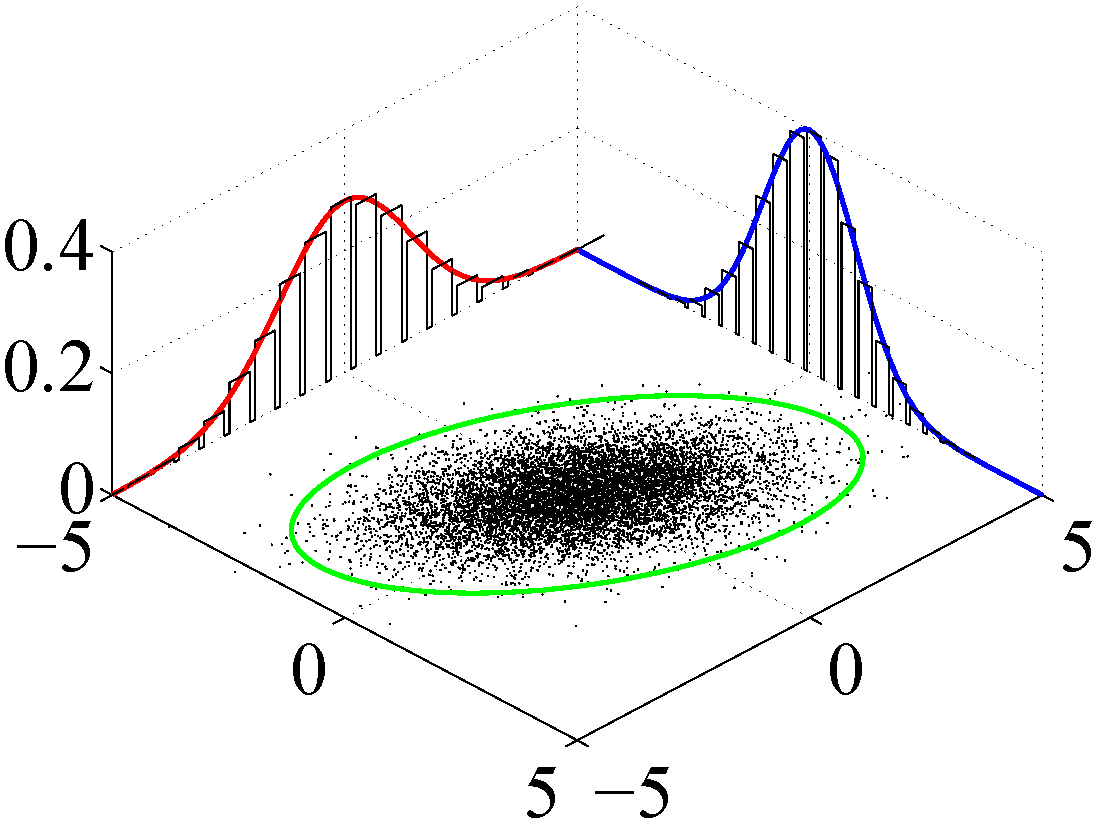
\includegraphics[width=\textwidth]{../figures/Multivariate_normal_sample.pdf}
  \end{column}

 \end{columns}
 
\end{frame}

\begin{frame}
 \frametitle{Uniform distribution}
 
 \begin{block}{Uniform distribution}
  For $x \in [a,b]$:
  
  $$f(x) = \frac{1}{b-a}$$
 \end{block}

 \begin{block}{Properties}
  \begin{itemize}
   \item Mean: $E(x) = \frac{b-a}{2}$
   \item Variance: $V(x) = \left(\frac{b-a}{12}\right)^2$, i.e. standard deviation $\sigma(x) = \frac{b-a}{\sqrt{12}}$
  \end{itemize}

 \end{block}

 
\end{frame}

\begin{frame}
 \frametitle{$\chi^2$ distribution}
 
 \begin{block}{$\chi^2$ distribution}
  $$f(x) = \frac{\frac{1}{2} \left( \frac{x}{2} \right)^{\frac{N}{2}-1} e^{-\frac{x}{2}}}{\Gamma(N/2)}$$
 \end{block}
  
 \begin{columns}
  \begin{column}{0.6\textwidth}
   
 \begin{block}{Properties}
  \begin{itemize}
   \item Mean: $E(x) = N$
   \item Variance: $V(x) = 2N$
  \end{itemize}
 \end{block}
 
 Example: sum of independent variables normally distributed ($t_N = \sum_{i=1}^{N} x_i^2$)
  \end{column}
  \begin{column}{0.4\textwidth}
   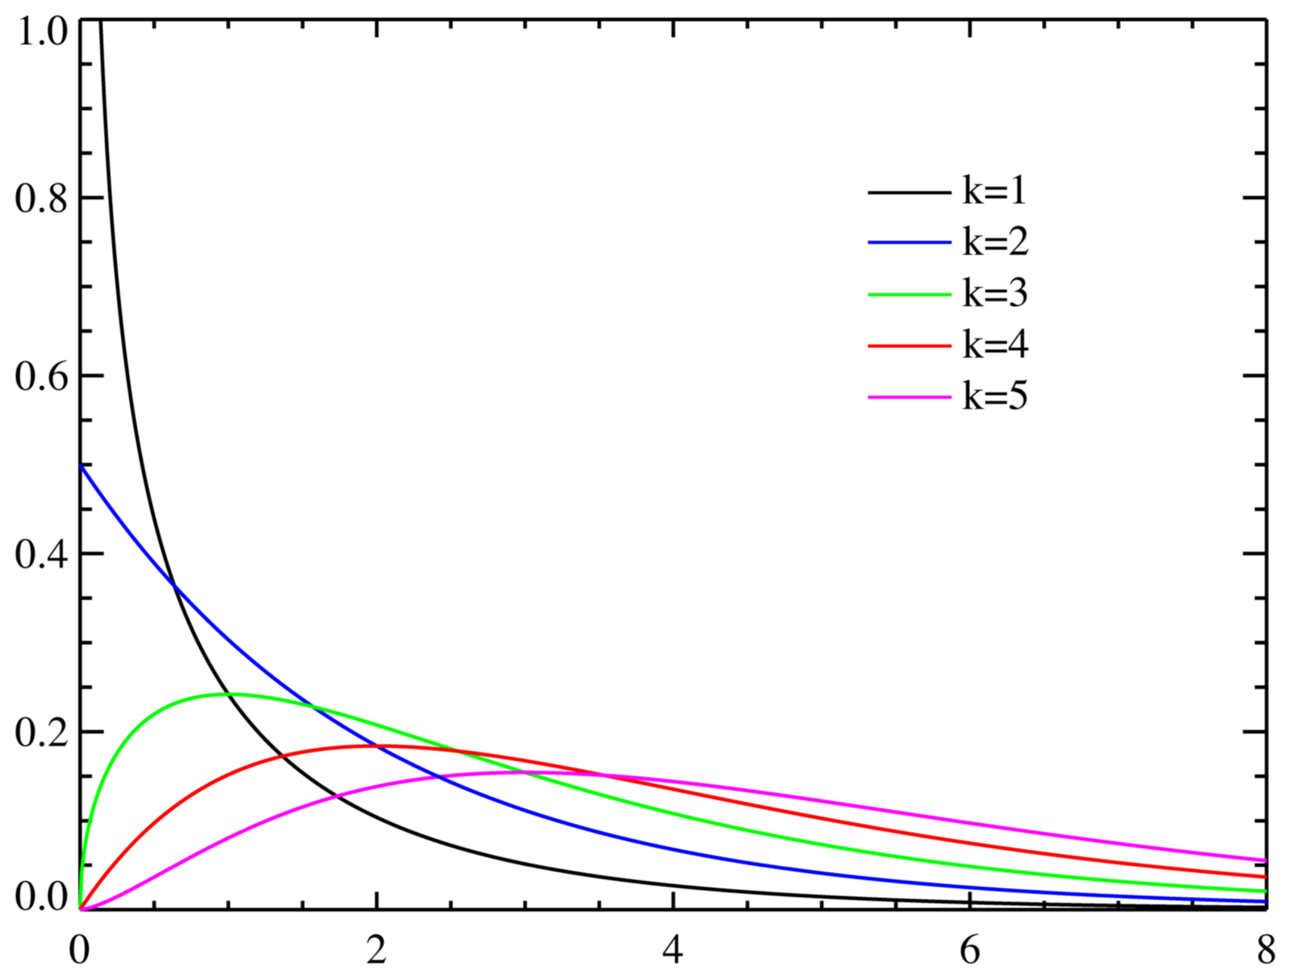
\includegraphics[width=\textwidth]{../figures/Chi-square_distributionPDF.png}
  \end{column}

 \end{columns}


\end{frame}


\begin{frame}
 \frametitle{Other distributions}
 
 \begin{description}
  \item[Cauchy distribution] (or Breit-Wigner): wider than a Gaussian, with undefined moments
  \item[Student's $t$]: kurtosis $>0$ (Cauchy is a special case of Student's $t$)
 \end{description}

\end{frame}

\section{Asymptotic theorems}

\begin{frame}
 \frametitle{Outline}
 
 \tableofcontents[current]
\end{frame}

\begin{frame}
 \frametitle{Asymptotic approach}
 
 Go back to the binomial law: $$B_{N,p}(n) = \frac{N!}{n!(N-n)!} p^n (1-p)^n$$
 
 Let us define $f_N = \frac{n}{N}$
 
 Then: $\langle f_N \rangle = \frac{pN}{N} = p$, $\sigma^2_{f_N} = \frac{p(1-p)}{N} \xrightarrow[N \to +\infty]{} 0$
 
 \begin{block}{Frequentist probability}
  $$\text{Frequentist } p \equiv \lim_{N \to \infty} \frac{n}{N}$$
 \end{block}

\end{frame}

\begin{frame}
 \frametitle{Law of large numbers}
 
 \begin{block}{Definition: convergence in probability}
  A sequence $\{X_n\}$ of random variables converges in probability towards the random variable $X$ if for all $\varepsilon > 0$

    $$ \lim _{n\to \infty }P \left( |X_{n}-X|>\varepsilon \right)=0$$
 \end{block}

\end{frame}

\begin{frame}
 \frametitle{Law of large numbers}
 
 Let $\{X_N\}$ be a sequence of random variables, such that $\forall i, \langle x_i \rangle = \mu$ and $\sigma^2_i = \sigma^2$. 
 
 We also define the sample mean
 $\bar{x} \equiv \sum_{i=1}^N \frac{x_i}{N}$
 
 \begin{block}{Weak law of large numbers}
  $$\text{If } \lim_{N \to \infty} \left( \frac{1}{N^2} \sum_{i=1}^N \sigma^2_i\right) = 0\text{, then } \bar{x} \xrightarrow[N \to \infty]{} \mu$$
  
  where the convergence is ``in quadratic mean''
 \end{block}
 
 \begin{block}{Strong law of large numbers}
  $$\text{If } \lim_{N \to \infty} \left( \frac{1}{N^2} \sum_{i=1}^N \sigma^2_i\right)\text{ stays finite, then } \bar{x} \xrightarrow[N \to \infty]{} \mu$$
  
  where the convergence is ``almost certainly''
 \end{block}
 
 Both imply convergence in probability.

\end{frame}



\end{document}

